\documentclass[12pt, floatsintext, jou]{apa6}
\usepackage{amssymb}
\usepackage{graphicx}
\usepackage[outdir=./]{epstopdf}
%\DeclareGraphicsExtensions{.eps}

\usepackage{mathtools}
\usepackage{enumerate}
\usepackage{apacite}
\usepackage{listings}
\usepackage{multirow}
\usepackage{todonotes}
\usepackage{svg}

\newcommand{\den}[2][]{
\(
\left\llbracket\;\text{#2}\;\right\rrbracket^{#1}
\)
}


\newcommand{\KL}[2]{\ensuremath{D_{KL}({#1}\, \| \, {#2})}}
\newcommand{\E}[2]{\ensuremath{\mathbb{E}_{#1}\left [#2 \right]}}

\newenvironment{figurehere}
	{\def\@captype{figure}}
	{}

\usepackage{lipsum}
%\pagenumbering{gobble}
%\usepackage{apacite}

\linespread{1}
\usepackage{textcomp}
\usepackage{lingmacros}

\DeclareGraphicsRule{.tif}{png}{.png}{`convert #1 `dirname #1`/`basename #1 .tif`.png}
\graphicspath{{./figures/}}
 
 \definecolor{Green}{RGB}{10,200,100}
\newcommand{\ndg}[1]{\textcolor{Green}{[ndg: #1]}}  


\makeatother

\title{Questions and answers in dialogue}
\shorttitle{Q\&A}
\author{Robert X.D. Hawkins, Noah D. Goodman}
\affiliation{Stanford University} 


\abstract{What makes a question useful? What makes an answer helpful? 
Linguistic theories have highlighted \emph{goal-relevance} as a key to explaining the function of questions and answers in dialogue. 
In this paper, we extend recent probabilistic cognitive models of goal-relevant communication to dialogue: agents hear an utterance, update their beliefs through social reasoning, and select an utterance in response.
The utility of producing a question in this framework is the expected reduction in uncertainty about the aspects of the world relevant to the speaker's goal. 
Critically, this suggests that the question itself can be a signal to the speaker's underlying goals, and that a helpful answerer should be informative with respect to \emph{inferred} goals, beyond the literal meaning of the question. 
We compare models within this framework based on three different pieces of evidence: 
First, we examine classic effects in psycholinguistics showing that the same question can yield different answers depending on the relevant goal in context.
Second, we run a real-time, multi-player communication game to jointly test predictions made by the questioner and answerer components of our model.
Third, we show that the \emph{salience} of goals affects both asking and answering questions.
We find that sophisticated pragmatic reasoning in dialogue is needed to account for critical aspects of the data.
}

\keywords{pragmatics, language, computational modeling, active learning, questions, answers}

\authornote{This report is based in part on work presented at the 37th Conference of the Cognitive Science Society. The first author is supported by a NSF Graduate Research Fellowship and a Stanford Graduate Fellowship. Correspondence concerning this article should be addressed to Robert X.D. Hawkins, e-mail: rxdh@stanford.edu}

\begin{document}
\maketitle
\section{The pragmatics of asking and answering}
Asking questions is one of our most valuable methods of gathering information and learning from others. 
At a very young age, children can strategically select \emph{who} to ask \cite{LegareEtAl13_QuestionsChildhood} and \emph{what} to ask \cite{Chouinard07_ChildrenQuestions, RuggeriLombrozo15_ChildrenAdaptQuestions} in order to solve problems and test lay theories \cite{CallananOakes92_PreschoolerQuestions, GopnikMeltzoffKuhl99_ScientistCrib}. 
Robots that ask questions to clarify commands \cite{DeitsTellex___Roy13_HumanRobotDialog} or obtain assistance with a task \cite{FongThorpeBaur03_RobotQuestions} make for better collaborators. 
In tutoring scenarios, students who ask better questions tend to be more successful \cite{GraesserPerson94_QuestionAskingTutoring}, and scientists who design their studies to ask better questions can obtain much more informative results \cite{ClarkSchober92_InfluencingAnswers, MyungPitt09_OED}.

A question is only as useful as its answer, however, and not all answers are created equal. How, then, does an answerer select from the broad range of possible responses? This is straightforward in some cases. For direct, factual questions, for example, an answerer can use the explicit meaning of the question, which specifies a particular gap in the questioner's knowledge, and respond with the requested piece of information if it is known: 
\enumsentence{
	Q: Who was the 16th president of the U.S.?\\
	A: Abraham Lincoln.}
This response strategy has been implemented in sophisticated semantic parsers that extract the logical form of the query and efficiently search a database for an entity that satisfies it \cite<e.g.>{BerantChouFrostigLiang13_FreebaseQAPairs}. 

Many questions in everyday conversation, however, are not so straightforward to answer. 
For a class of questions called indirect speech acts, the questioner typically will not be satisfied with a simple yes/no answer; they expect the answerer to go \emph{beyond} the literal meaning to address the questioner's true interests \cite{Clark79_IndirectSpeechActs}:  
\enumsentence{
	Q: Do you know the time?\\
	A: It's a quarter past 3.}
%\enumsentence{
%	Q: Do you know how to get to the campus bookstore?\\ 
%	A: It's on the other side of campus, but there's a shop just down the street with a better selection.}
 
Indeed, answerers often go beyond the literal meaning even for \emph{direct} questions. A recent corpus study found that 14\% of responses to direct yes/no questions used a full statement instead of a simple ``yes'' or ``no'' \cite{DeMarneffeGrimmPotts09_IndirectAnswersCorpus}:

\enumsentence{
	Q: Is it in Dallas?\\
	A: Uh, it's in Lewisville.}

Finally, there's a class of questions familiar to any classroom instructor, where the questioner apparently doesn't even know what their true interests are:

\enumsentence{
	Q: What's wrong with my answer to \#1?\\ 
	A: Well, let me remind you how to compute a derivative...}

 What do these exchanges have in common? Q strategically chooses a question that manages to send a signal to A about her intentions, while sometimes being unable or unwilling to specify exactly what those intentions are. They may be impolite or embarrassing, they may be too long or costly to fully explain, or she may just not know enough about the topic she's interested in to articulate them.

A, in turn, reasons beyond the overt question and provides an answer that addresses Q's true interests. Depending on the circumstances, he can adjust his response to be over- or under-informative with respect to the direct question, or to address a different question altogether.  This subtle interplay between a questioner choosing a question to ask and an answerer choosing  a response raises two specific questions for formal models of language behavior: What makes a question useful? And what makes an answer helpful? 

We suggest, following \citeA{VanRooy03_QuestioningDecisionProblems}, that the value of a question is the extent to which it can be expected to elicit useful information from an answerer. 
More specifically, for the questioner, the value of a question is the expected information gained relevant to her interests, given the set of likely answers it may provoke. The value of an answer, then, is the extent to which it resolves questioner uncertainty over the goal-relevant aspect of the world. 

Our contribution in this paper is threefold. First, while psychologists have learned quite a bit about questioner behavior and answerer behavior by studying the two processes in isolation, we argue that there are significant theoretical benefits in viewing them as deeply intertwined social inferences. Second, we formalize this theoretical view of question-answer behavior in a probabilistic model of language understanding as social reasoning. This is the first time that such language models have been extended beyond single utterances and hence provides a first step toward modeling longer dialogues. Third, we address a longstanding paucity of data on \emph{questioner} behavior by running a set of real-time, multi-player communication games in which we simultaneously observe both ends of the dialogue. 

%

The rest of this paper is structured as follows. First, we review previous experimental results and formal models from the question-asking and question-answering literature. We then lay out the details of our computational approach  to questioner and answerer models, including several variants of each. We present a set of computational experiments demonstrating how this set of models captures four classic answerer-sensitivity effects.
%we specify a family of questioner and answerer agents, highlighting some points of divergence from previous RSA models. 
%We then formally individuate literal, explicit, and pragmatic models in this family, which represent different hypotheses about how questioners and answerers reason about their task. 
%In particular, we compare a pragmatic answerer making inferences about the questioner's goals to two simpler models: one that takes into account only that an answerer wants to be maximally informative with respect to the explicit question asked (without inferring the questioner's underlying decision problem) and one that provides a literal answer to the question (without attempting to be maximally informative).  
Because data on \emph{questioner} behavior is relatively sparse, and these classic results did not sufficiently test the questioner component of our model, we collected data in a real-time, multi-player communication task allowing us to manipulate private goals, potential questions, and potential answers. After testing the predictions of the different models on data from a simple version of the task, we use our models to discover conditions that disambiguate our hypotheses in a second experiment using a wider set of stimuli.
We close with a brief discussion of how our approach grounds question-asking and answering in social cognition, noting the potential scalability of our framework to more complex discourse contexts, natural language understanding, and active learning.


\subsection{Empirical background}

A number of psycholinguistic studies have provided evidence that answerers are both sensitive to a questioner's goals and attempt to be informative with respect to those goals.
For instance, in Clark's \citeyear{Clark79_IndirectSpeechActs} classic study, researchers called liquor merchants and asked ``Does a fifth of Jim Beam cost more than \$5?'' Before asking the question, they provided some context for their call by saying either ``I want to buy some bourbon'' (the \emph{uninformative} condition) or ``I've got \$5 to spend'' (the \emph{five dollar} condition). 
These contexts signaled different speaker goals. In the uninformative condition, the goal is simply to buy whiskey, hence the exact price would be useful information; in the five dollar condition, the goal was literally to find out whether or not the speaker could \emph{afford} the whiskey, so a yes/no answer would suffice. 
If merchants inferred these goals from the context signal and responded with respect to these goals, we would expect different types of answers in the two conditions. Indeed, merchants gave a literal yes/no answer significantly more often in the latter condition than the former, where an exact price was more common. 

Goals can also be inferred from non-linguistic environmental cues. For instance, \citeA{DerHenstCarlesSperber02_RelevanceTellingTime} investigated answers to questions like ``Do you have the time?'' that permit answers with different degrees of approximation to the true time \cite<see also>{GibbsBryant08_OptimalRelevance}. In a baseline condition, participants who were approached in public typically rounded their answers to the nearest 5 or 10 minute interval even when they were wearing a digital watch. 
%This showed that answerers were not simply reducing their \emph{own} effort, since rounding a time displayed on a digital watch requires an extra processing step. 
When the experimenter mentioned that they had an appointment at a given time, however, they found that answers were more likely to be precise when the true time was closer to the appointment time, indicating sensitivity to implicit time-related goals such as knowing whether to hurry.  
%In a later study,  introduced a condition in which this question was preceded by the statement ``My watch stopped,'' and found that answerers were more likely to make their response precise to the minute. 
%An approximate time is sufficiently informative with respect to most common goals, like making it to a meeting on time, yet answerers were able to adjust their response after inferring a less common goal, like setting a watch, which required more precise information.

% investigated the relationship between questioner goals and answerer sensitivity using the Cards corpus, a collection of transcripts and associated contextual information from a two-person collaborative game. 
%In the game, two players were placed in a virtual world where they were instructed to collect cards with six consecutive numbers from the same suit. Each player could only hold three cards at a time, and neither player could see the other, thereby requiring the players to explicitly coordinate their locations. 
%Using an information-theoretic measure to quantify a response's degree of specificity, Potts found that answers tended to be more specific when the questioner was trying to meet up or direct the answerer to a specific card, and less specific when developing a general search strategy. 

Linguists interested in pragmatic accounts of answerer behavior have noted a number of additional scenarios with more nebulous goals. Questions like ``where are you?'' permit answers at many degrees of specificity: \emph{the United States}, \emph{my apartment}, and \emph{by the big tree} are each perfectly appropriate in some context and highly inappropriate in others \cite{Potts12_CardsDialogueCorpus}. Identification questions like ``who is X?'' can be resolved in many ways  \cite{BoerLycan75_KnowingWho, Gerbrandy00_Identity, Aloni05_ConceptualCovers}. 
For example, if an undergraduate asked ``Who is Noam Chomsky?'' in an introductory course, it would be appropriate to respond ``The MIT professor who wrote \emph{Aspects of the Theory of Syntax}'' or ``The father of modern linguistics.'' If a potential donor asked the same question at an MIT fundraiser, though, it would be more appropriate to point at Chomsky in the crowd. 
Similarly, if a child asks ``What's that?'' while pointing at a common household object, a parent's response will be much different than if one of their adult friends asked the same question. More specific \emph{wh}-questions like ``Who passed the examination?'' have also been studied extensively in developing linguistic theories: answers can be understood to mean either an \emph{exhaustive} or \emph{selective} list of relevant entities \cite{SchulzVanRooij06_ExhaustiveInterpretation}.

% "WHY ARE WE DOING THIS?" paragraph
Taken together, this body of work suggests that \emph{goal-relevance} is a critical feature of question-answering: answerers routinely go beyond the literal meaning of a question to help the questioner achieve their underlying goals. Note that the vast majority of prior work on question-answer behavior has focused on the \emph{answerer}, holding the question constant and investigating the effect of different contexts. 
However, questioners must also select between many alternative questions in order to achieve their goal, and their utterance serves as a signal that prompts a relevant response from the answerer. Next, we review a set of formal proposals about the questioner's role in dialogue.  

\subsection{Modeling background}

An artificial agent capable of flexibly answering questions posed in natural language would be valuable for a diversity of practical applications, from customer service and technical support to health care and financial consulting. It's no surprise, then, that the problem of question-answering has attracted attention from researchers in the artificial intelligence community for decades \cite{Simmons65_QuestionsComputer, Lehnert77_QuestionAnswering, AllenPerrault80_IntentionUtterances, GreenCarberry94_IndirectAnswersModel, MollaVicedo07_QARestrictedDomains}. Some of these systems are highly domain-restricted interfaces for databases, such as the kind that could be used to show airline customers flights that meet their criteria, but many build on insights from early work in cognitive science to represent questioner intentions as schemas or plans. For instance, the system designed by \citeA{AllenPerrault80_IntentionUtterances} uses a set of logical rules to generate a space of possible plans, searches this space using a set of heuristics, identifies obstacles to fulfilling this plan, and takes a set of actions to address the obstacles. 

While AI researchers were building automated systems to answer questions, linguists were developing formal theories of what questions and answers meant in the first place, mainly focusing on the notion of informativeness. In Groenendijk and Stokhof's \citeyear{GroenendijkStokhof84_SemanticsOfQuestions} foundational work on question and answer semantics, asking a question induces a partition over the space of possible worlds, where each cell of the partition corresponds to a possible answer. An answer, then, consists of eliminating cells in this partition, and the most useful answers are those that eliminate all relevant alternatives to the true world. However, as van Rooy \citeyear{VanRooy03_QuestioningDecisionProblems} and others \cite{Ginzburg95_ResolvingQuestions} have pointed out, this predicts that wh-questions like ``Where do they sell Italian newspapers in Amsterdam?'' can only be fully resolved by exhaustively mentioning whether or not such a newspaper can be bought at each possible location in the city. Clearly, this is not the case: a single nearby location would suffice. These theories also cannot account for contextual variation in what counts as a useful answer: if a media executive asked this same question at a corporate meeting, they might legitimately be requesting an exhaustive list.

More recent theories have tried to fix these problems by introducing some consideration of the questioner's goals. \citeA{VanRooy03_QuestioningDecisionProblems}, for instance, formalizes these goals in terms of a decision problem faced by the questioner and assumed to be in common ground. He considers two proposals for how meanings depend on this decision problem, ultimately arguing for the second. 

In the first proposal, questions have a context-independent meaning -- in the sense that an interrogative sentence always creates the same partition on worlds -- but the extent to which an answer is \emph{useful} or \emph{resolving} is determined by the decision problem. In particular, a useful answer under this account is one that maximizes the expected value of the questioner's decision problem, even if it is not a complete semantic answer. 

In the second proposal, the meaning of a question is \emph{underspecified} and its interpretation depends on the decision problem. In particular, because the questioner is assumed to be rational, the answerer chooses the interpretation that would maximize the expected value of the answer. We take these proposals as a starting point for the meaning of questions in our model.

\section{A Rational Speech Act model of \\questions and answers in dialogue}

\subsection{Overview}

% WHAT PROBLEMS NEED TO BE SOLVED IN DIALOGUE?
%We begin by presenting a general computational framework for agents in dialogue, then focus on the problem of question-asking and answering in particular. 
Broadly speaking, an agent must solve two problems to participate in a dialogue. First, they must \emph{listen}, interpreting the meaning of their partner's utterance and updating their own beliefs accordingly. Then they must \emph{speak}, producing an utterance that informatively addresses the current goal or topic of conversation. At either stage, the utterance may be a statement, a question, or another more exotic kind of speech act. 

\begin{figure*}[t]
\begin{center}
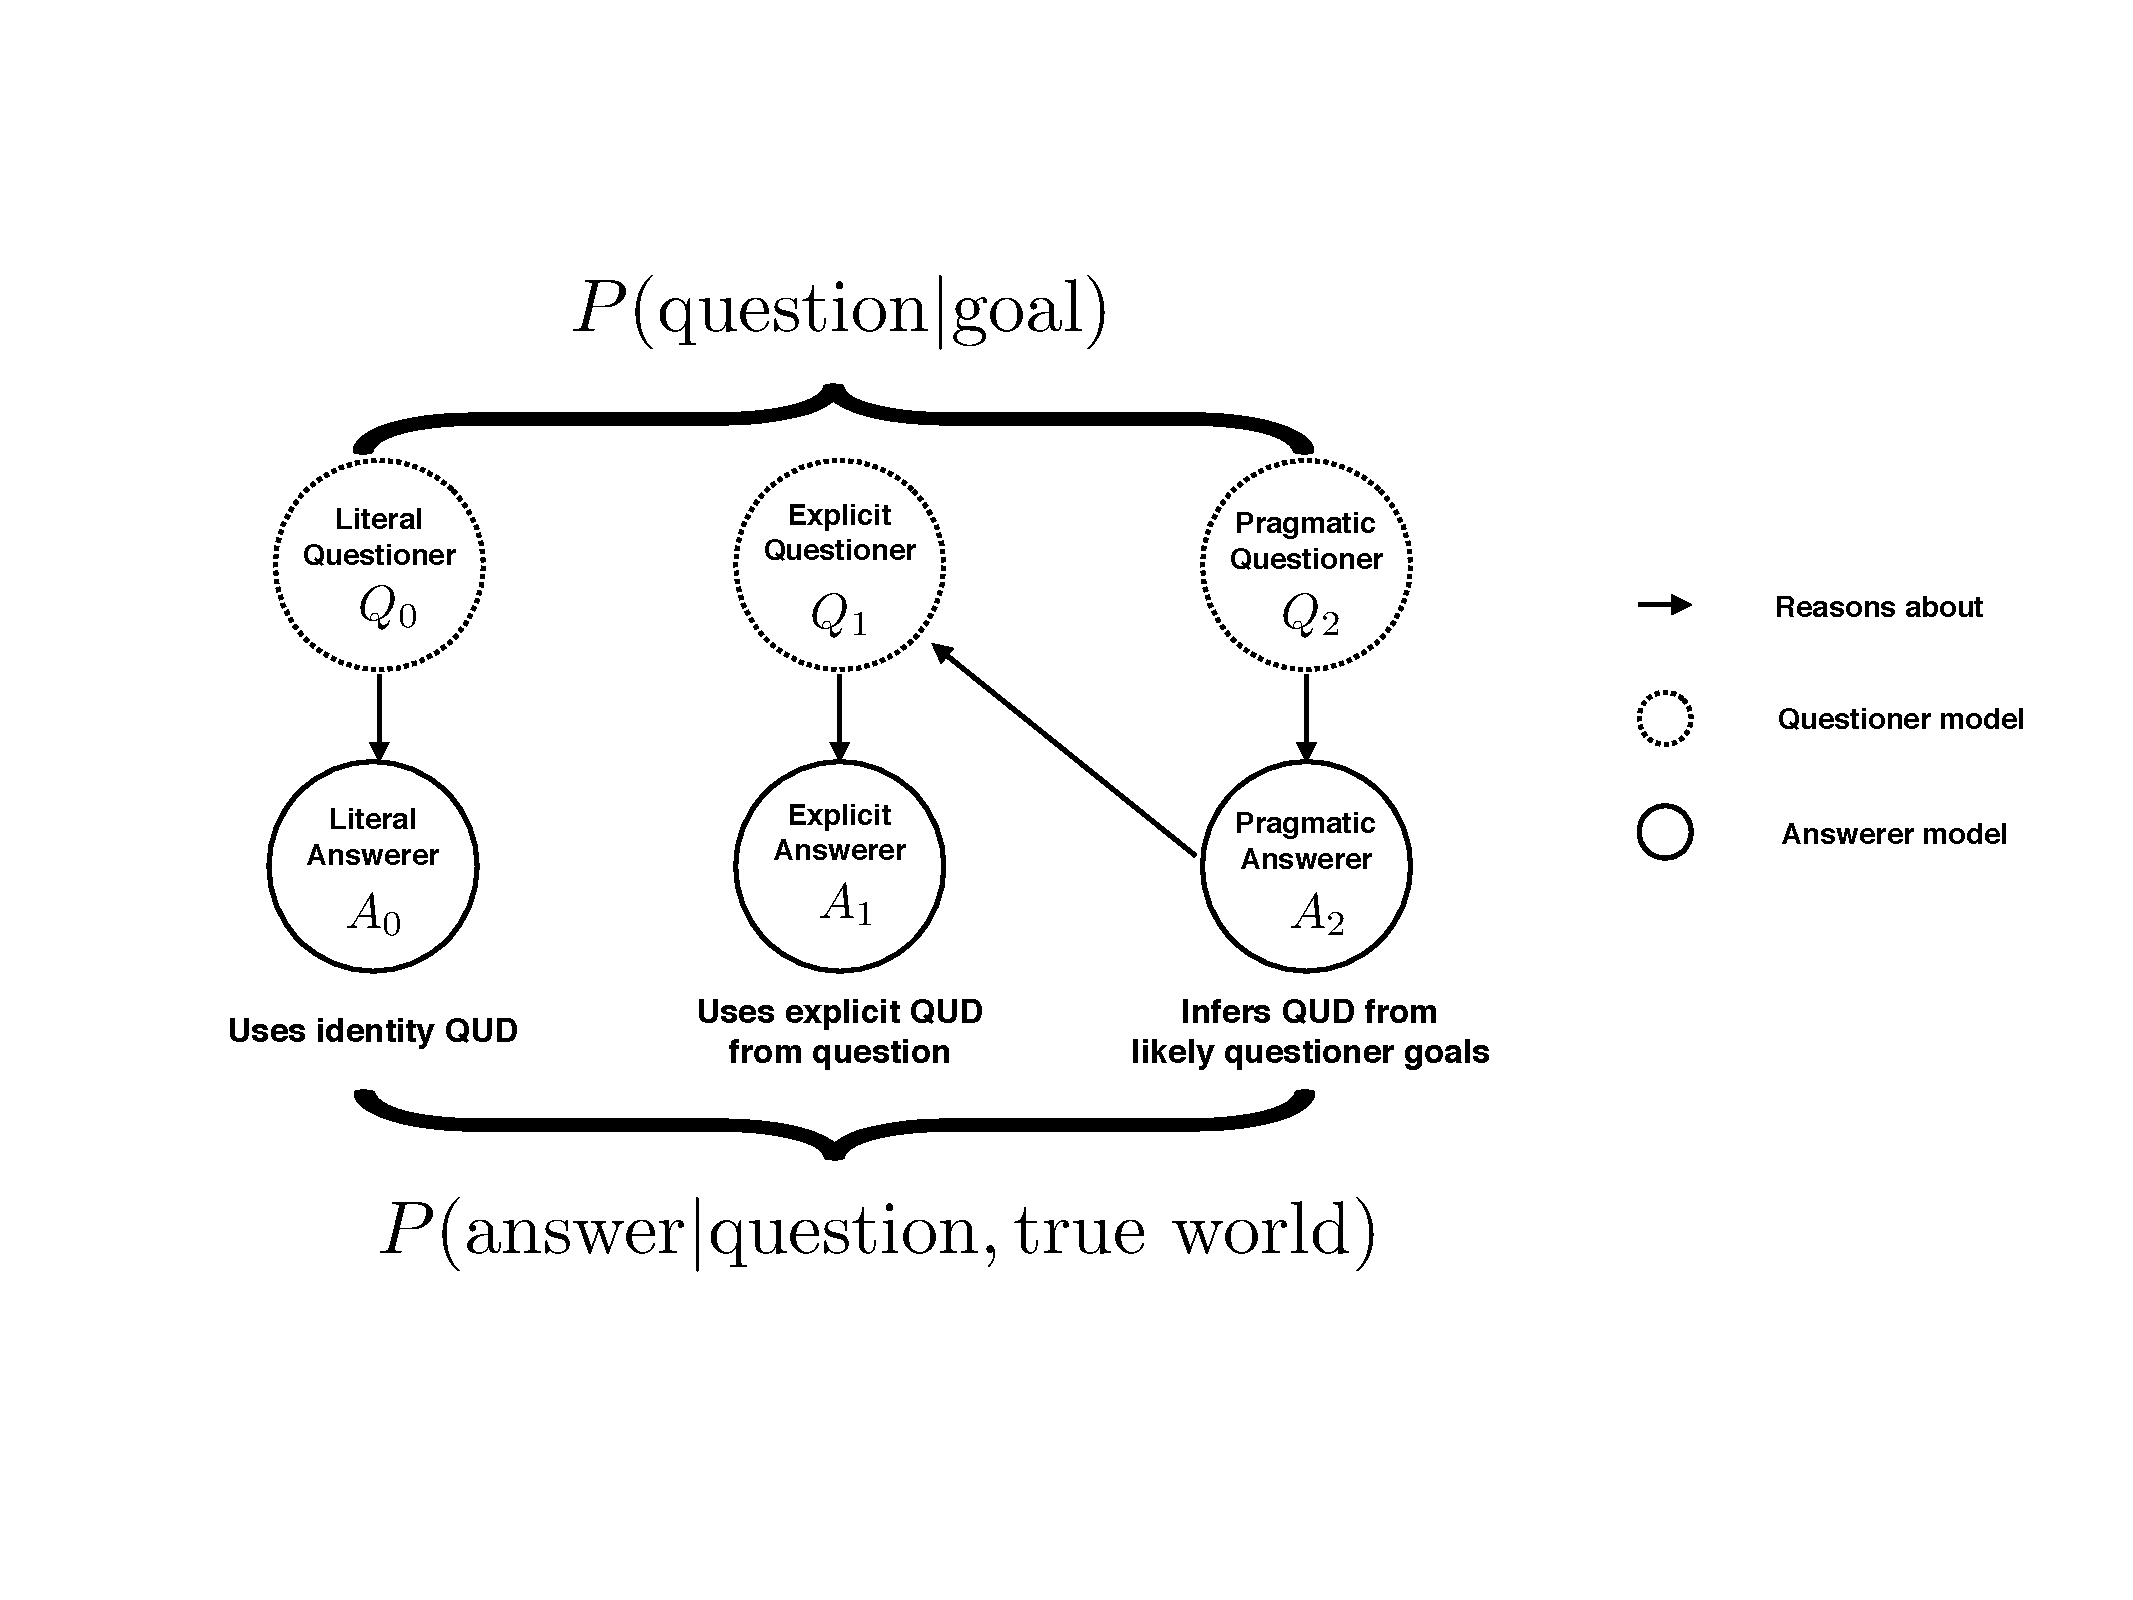
\includegraphics[scale = .5]{models.pdf}
\end{center}
\caption{Schematic of the questioner and answerer models we consider, showing their recursive relationships. Note that there are two possible ``base cases'' where the recursion can terminate: in a \emph{literal} answerer that ignores the question and simply attempts to be informative with respect to the world, and in an \emph{explicit} answerer that uses the semantics of the questions. \ndg{put $P_I$ in this fig?}}
\label{fig:models}
\end{figure*}

% HOW ARE THESE ADDRESSED IN RSA?
Both the listening problem and the speaking problem have been addressed within the Rational Speech Act (RSA) framework \cite{FrankGoodman12_PragmaticReasoningLanguageGames, GoodmanStuhlmuller13_KnowledgeImplicature, GoodmanFrank16_RSATiCS}, in which language understanding is formalized as recursive Bayesian inference. Pragmatic speaker agents choose utterances to maximize their partner's surprisal about the true state of the world -- a basic epistemic goal -- and pragmatic listener agents interpret utterances by inverting the speaker model. This basic framework has been used to account for a number of diverse pragmatic phenomena including 
scalar implicature \cite{GoodmanStuhlmuller13_KnowledgeImplicature}, %prosody \cite{BergenGoodman15_StrategicUseOfNoise},
%the acquisition of word meanings \cite{FrankGoodman14_InferringWordMeanings}, and
generic language \cite{TesslerGoodman16_Generics}, and
interpretation of context-sensitive adjectives like ``tall'' or ``cheap'' \cite{LassiterGoodman15_AdjectivalVagueness}.

% HOW IS GOAL-RELEVANCE FORMALIZED IN RSA?
RSA models have also recently been extended to incorporate the critical notion of \emph{goal-relevance} into the speaker's utility \cite{Roberts96_InformationStructureDiscourse, WilsonSperber12_MeaningRelevance}. Instead of attempting to be maximally informative about the \emph{full} state of the world, the speaker ignores irrelevant dimensions and only attempts to be informative about the relevant feature or summary statistic. RSA models with relevance have been used to capture non-literal language use like hyperbole \cite{KaoWuBergenGoodman14_NonliteralNumberWords}, metaphor \cite{KaoEtAl2014-Cogsci}, or irony \cite{KaoGoodman15_IronyCogSci}. In the case of hyperbole, for instance, a speaker who says ``It took a million years to get a table'' may be intending to be informative about the topic of their affective state rather than the exact time it took to get a table. 

% HOW IS OUR MODEL DIFFERENT FROM PAST MODELS (DIALOGUE!)
Our model builds upon these recent modeling advances in several novel ways. 
First, by unifying the listening problem and speaking problem in a single rational agent, we provide a principled cognitive connection between linguistic input and output: different kinds of input shift an agent's beliefs in different ways, motivating different kinds of responses. 
%This is a first step toward chaining together more complex multi-utterance discourse phenomena.

% HOW IS OUR MODEL DIFFERENT FROM PAST MODELS (QUESTIONS!)
Additionally, questions have previously posed a challenge for rational models of language use, since questions -- as utterances -- don't provide direct information about the world to the listener.
The crucial motivation to ask questions in the first place, of course, is an asymmetry between speaker and listener knowledge; agents have \emph{private goals} in addition to private knowledge about the true state of the world. 
%\footnote{That is, the literal meaning of a question does not seem to be new information about the world, per se. Questions do, of course, end up conveying information about the speaker's knowledge, needs, and so on---it is this conveyed information that we attempt to derive below.}. 
While a declarative statement in our framework provides evidence about the true state of the world, we conjecture that a question provides evidence about the \emph{speaker's goals}. 

Rather than defining the meaning of a question in terms of its possible answers, as in traditional linguistic theories, we treat it as a \emph{signal} that the listener can use to update their beliefs about the speaker's goals. 
When it is the listener's turn to speak, they can then generate statements that address the goal-relevant aspects of the world. In the next section, we review the basic RSA framework and explore several different proposals for how agents interpret and respond to questions within this framework.
 %This diverges from previous RSA models in that the value of a question depends on information gained by the speaker (rather than listener), and that this information comes later in the (very short) conversation. 



%The account of questioner and answerer behavior we propose in this section is a an effort to synthesize linguistic theories of question semantics with rich, quantitative cognitive models of language understanding. 
%We jointly model the questioner's choice of question and the and answerer's choice of answer through recursive social reasoning, allowing the answerer to \emph{infer} the questioner's private goal from observing the context and question utterance. 

%If the questioner determines what question to ask by reasoning about likely answers, we must specify what kind of answerer they are reasoning about. We explore three increasingly sophisticated kinds of answerers, which serve as possible internal models used by the questioner, yielding three increasingly sophisticated kinds of questioners; these three models serve also independently as models of actual answerers. 
%The simplest agent, the literal answerer, simply attempts to be maximally informative about the true state of the world, ignoring the question;   
%the explicit answerer assumes that the question has a context-independent meaning and attempts to be informative with respect to that meaning (without inferring the questioner's underlying interests);  
%the pragmatic answerer treats the question as a signal to the questioner's underlying goals, infers the most likely underlying interests of the questioner, and then informatively addresses those interests (see Figure \ref{fig:models})\footnote{In terms of \citeA{VanRooy03_QuestioningDecisionProblems}, the meaning function used in the explicit models corresponds to the first proposal of context-independent semantics, while our pragmatic models roughly correspond to the second.}. 
%The latter model uses an extension of RSA to reason about the topic of conversation, as proposed by \citeA{KaoWuBergenGoodman14_NonliteralNumberWords}; it goes beyond previous work by using the explicit question as a (potentially indirect) cue to this topic. 

\label{sec:model}

\subsection{Preliminaries}

Our mathematical formalization of dialogue begins with four primitive sets that agents take to be in common ground. For concreteness, we use the scenario from \citeA{Clark79_IndirectSpeechActs} as an example throughout: 
\begin{description}
\item[$\mathcal{W}$:] a set of true states of the world, such as the true price of a bottle of whiskey \{\$1, \$2, \dots, \$10\}. In principle, this may also include other features of the world, such as the current weather, the location of nearby caf\'es, or the kinds of payment that the store accepts.
\item[$\mathcal{G}$:] a set of possible underlying questioner goals, such as learning the actual price of the whiskey or learning whether or not one can afford to buy the whiskey at all. 
We formalize the key notion of an informational goal $g \in \mathcal{G}$ as a projection function $g: \mathcal{W} \rightarrow \widehat{\mathcal{W}}$ that maps a world state $w$ to a particular feature or set of features that the questioner cares about, which we denote $\widehat{w} = g(w)$; this is similar to the notion of a question-under-discussion \cite<QUD;>{Roberts96_InformationStructureDiscourse}. For example, the customer's goal of learning the actual price of the whiskey is given by the identity function $g_{=}(w) = w$, while the goal of learning whether it is affordable is given by 
$$g_{<}(w) = \left\{\begin{array}{rcl}
1 & & w < 5 \\
0 & & \textrm{otherwise}
\end{array}\right.$$
such that all worlds where the agent can afford the whiskey are mapped onto one state, and all other words are mapped onto a different state.
\item[$\mathcal{Q}$:] a set of possible question utterances , such as ``Does a fifth of Jim Beam cost more than \$5?'' or alternatives like ``Do you accept credit cards?'' We take the literal meaning \den{$q$} of a question to be of the same type as informational goals, such that a particular question utterance corresponds to a particular goal projection\footnote{This is equivalent to the more common partition semantics of \citeA{GroenendijkStokhof84_SemanticsOfQuestions}, as can be seen by considering the pre-image of such a question projection: $q^{-1}(\hat{w})$.}. For example, the literal meaning of the question ``Does a fifth of Jim Beam cost more than \$5?'' is a function that maps all worlds $w$ such that $w > \$5$ to one value and all other worlds to a different value. Note that the correspondence between questions and goals is not necessarily symmetric: while every question corresponds to a goal, we do not expect that every possible goal corresponds to a question utterance.
\item[$\mathcal{A}$:] a set of possible declarative utterances, such as ``It costs \$7.'' or ``Yes, it costs more than \$5.'' We take the literal meanings of these declarative utterances \den{$a$} to be truth-conditional: a map from world states to booleans. For instance, the utterance ``A fifth costs \$8.'' would be true in the world where $w = \$8$ and false otherwise. 
\end{description}
%QUDs are often used in formal linguistic models to capture \emph{relevance}: there are many informative sentences one can use to convey a full world state, but only a few of those are informative with respect to the current topic of discussion. \ndg{this comment about relevance seems out of place.}

\subsection{$A_0$: Informative Answerer}

We begin by considering the problem of how a dialogue agent ought to interpret and respond to a question utterance. The simplest baseline answerer, $A_0$, attempts to be informative about the state of the world without considering his partner's goals. In other words, $A_0$ is a rational speaker without any corresponding listener component to interpret and relevantly address its input. 

Formally, $A_0$ hears a question utterance $q \in \mathcal{Q}$ with private knowledge about the true world state $w \in \mathcal{W}$. He then uses a soft-max decision rule to choose an utterance $a \in \mathcal{A}$ proportional to the epistemic utility of that utterance to his communication partner: 
$$P_{A_0}(a | q, w) \propto \exp(\alpha U_{A_0}(a;w))$$ 
where $\alpha$ is a soft-max optimality parameter. 

We define the epistemic utility of the utterance using the information-theoretic measure of surprisal: the increase in an imagined interpreter $I$'s certainty about the true state of the world after hearing $a$: 
\begin{equation}
\label{eq:A0utility}
U_{A_0}(a;w) = \ln P_I(w|a)
\end{equation}

Critically, $A_0$ assumes that $I$ uses Bayesian inference to update their beliefs about worlds, conditioning on the literal meaning of the utterance $a$ being true:
$$P_I(w|a) = \delta_{\textrm{\den{a}}(w)} P(w)$$
where $\delta_{e}$ is the delta function returning 1 when $e$ evaluates to true and 0 otherwise, and $P(w)$ is a prior over true states of the world. 
%In other words, the interpreter constrains the prior on worlds to the subset of its support that is consistent with the given utterance, and $A_0$ attempts to (soft)-maximize the probability of the true world in this posterior. 

This formulation of $A_0$ is equivalent to the pragmatic speaker $S_1$ for declarative statements in previous RSA models \cite{GoodmanFrank16_RSATiCS}. It thus serves as a useful baseline model for several reasons: for one, it chooses utterances using the same basic utility as the more sophisticated models we consider, thus serving as a ``lesioned'' speaker to evaluate the necessity of the listener component. At the same time, it is a more charitable baseline than a purely random speaker: if asked about a fifth of Jim Beam knowing that it costs \$8, $A_0$ would prefer ``It costs \$8'' to ``It costs more than \$5'' or (falsely) ``It costs \$4'' simply because the former leads to an interpreter placing more probability on the true state of the world ($w = $ \$8).

%%%
%\footnote{For the purposes of this paper, we assume answers are always full sentences, corresponding to truth-functional propositions that can be evaluated in a given world. The interpreter described is the simplest required to model such answers. For fragments such as `yes' or `Bob,' which can be used to answer questions like `Is dinner at 7pm?' or `Who got the promotion?' we would require a more sophisticated interpreter that can compositionally expand the fragment into a valid proposition, using the question. This is a standard operation in formal semantic models, and an interesting target for future research, but is not necessary for the experiments we report.}

\subsection{$A_1$: Relevantly Informative Answerer}

While $A_0$ is informative, he is not particularly \emph{relevant}. When asked about the weather, he is just as likely to inform his partner about what he ate for breakfast as he is to say ``it's sunny.'' How do we incorporate relevance into the answerer's utility? 

Following \citeA{KaoWuBergenGoodman14_NonliteralNumberWords}, we formalize speaker relevance by means of a projection function. Instead of trying to increase the listener's certainty about the most fine-grained true world state, a relevant speaker only cares about the listener's certainty in a coarser space in which irrelevant features have been collapsed together. That coarser space is the image $\widehat{\mathcal{W}}$ of the goal-projection $g$.
%$$\widehat{P^g}(w') = \sum_{w\in\mathcal{W}} \delta_{w' = g(w)} P(w)$$ 
Thus, we modify the utility from Eq. \ref{eq:A0utility} to define a relevantly informative answerer $A_1$: 
$$U_{A_1}(a; g, w) = \ln \sum_{w' \in \mathcal{W}} K_g(w, w') P_I(w' | a)$$
where $K_g(w,w')$ is a similarity function (or kernel) between worlds, given by the goal. For the discrete space of goals considered in the current work, we use the delta function $K_g(w,w') = \delta_{g(w)=g(w')}$ which combines the probabilities of all worlds that map to the same value in $\widehat{\mathcal{W}}$\footnote{Note that $g$-projection is a generic operation on any probability distribution $P(w|\,\cdot)$, which we denote: 
$$\widehat{P}^g(w|\, \cdot) = \E{P(w'|\, \cdot)}{\delta_{g(w) = g(w')}}$$\todo[inline]{rdh: not 100\% satisfied with this notation}}.

%$$
%\begin{array}{rcl}
%U(a; g, w) & = & \ln \widehat{P^g_I}(g(w)|a) \\
%                 & = & \ln \sum_{w'\in\mathcal{W}} \delta_{g(w) = g(w')} P_I(w' | a) \\
%                 & = & \ln \sum_{w'\in\mathcal{W}} K_g(w,w')P_I(w' | a)
%\end{array}
%$$
This modified speaker component suggests a simple proposal for a corresponding listener component: we use the semantics of the question $q$ itself as the goal projection:
$$P_{A_1}(a|q,w) \propto \exp(\alpha U_{A_1}(a; q,w))$$
This implements one of the simplest plausible theories of answerers in dialogue: $A_1$ directly interprets a question as an epistemic goal, then informatively produces an utterance that reduces the questioner's uncertainty under that goal projection. 

$A_1$ may be sufficient for many simple, fact-based questions, like ``Who was the 16th president of the U.S.?'' given a rich enough semantic parser to supply the semantics of $q$ \cite{BerantChouFrostigLiang13_FreebaseQAPairs}. Still, the dazzling display of context-sensitivity and indirectness displayed in everyday communication suggests that deeper social reasoning may be at play. To explore more sophisticated answerers that reason about context and their partner's underlying goals, we must first address the problem of how a speaker chooses between questions.

\subsection{$Q_0$ and $Q_1$: Direct Questioners}

If the utility of uttering a declarative statement is imparting information about the true state of the world, what is the utility of uttering a question? We begin by assuming that a questioner aims to \emph{learn information relevant to a private goal}.
%
In order to choose a question that results in useful information, the questioner reasons about how her dialogue partner would respond in different possible states of the world. She then selects a question that results in an answer that tends to reduce her own uncertainty about goal-relevant information.
%

% This is a divergence from previous RSA models, where agents choose utterances with the goal of imparting information about the state of the world.

More formally, a questioner agent takes a goal $g \in \mathcal{G}$ as input and returns a distribution over question utterances $q \in \mathcal{Q}$ by solving a simple planning problem involving two components: (1) which answers are likely to come back after asking this question, and (2) how much would be learned from each of those answers. Critically, in order to solve either of these parts, the questioner must have in mind an imagined answerer who hears her question and responds appropriately: thus, we have a family of questioners $Q_i$, each using the corresponding answerer $A_i$:
%
$$
\begin{array}{lcl}
P_{Q_i}(q|g)  & \propto & \exp\{\alpha U(q;g)\} \\
U(q;g) & = & \E{P(a|q)}{IG^g(a,q)} \\
	 & = & \sum_{w\in\mathcal{W}} P_{A_i}(a|q,w)P(w) IG^g(a,q)
\end{array}
$$
%

The expectation over likely answers $P(a|q)$ is computed by running an imagined answerer model forward, marginalizing over the possible worlds $w \in\mathcal{W}$ they might have knowledge of. The likelihood of an answer weights its \emph{information gain} $IG^g(a,q)$: the gap between the questioner's beliefs about the $g$-relevant state of the world before and after hearing an answer. Drawing again upon information theory, we formalize the notion of information gain using the Kullback-Leibler divergence between the $g$-projected prior distribution and posterior after hearing $a$.
%
$$
IG^g(a,q) = \KL{\widehat{P^g}(w|q, a)}{\widehat{P^g}(w)}\\
$$
%

In order to anticipate her posterior beliefs after hearing an answer, the questioner must again make use of an imagined answerer, but now imagining herself as a listener in the future and inverting that model to infer the true world the answerer was trying to communicate:
$$P(w|q,a) = P_{A_i}(a| q, w)P(w)$$

Note that $Q_0$, who plans their question by reasoning about the likely responses of $A_0$, does not prefer any utterance over any other, because they will all lead to the same distribution of (informative) answers. $Q_1$, on the other hand, expects $A_1$ to directly interpret their question as a goal and respond informatively and relevantly, thus allowing for some questions to be better than others. Critically, in contrast to \cite{GroenendijkStokhof84_SemanticsOfQuestions} and \cite{,VanRooy03_QuestioningDecisionProblems}, the questioner's behavior is not governed fully by the semantics of the question she asks, but by what she actually expects her partner to say after hearing it.

\subsection{$A_2$: Goal-Sensitive Answerer}

%How should an answerer choose between answers to a question? What should a questioner assume about the answerer when choosing a question? We next describe three different answerer models; the questioner could assume any one of them, leading to three corresponding versions of the questioner model. From here on, we index the questioner and answerer models by $i$ to formulate different questioner models $Q_i$ which reason about different answerers $A_i$ (see Figure \ref{fig:models}).
%All answerers take a question $q \in \mathcal{Q}$ and a true world state $w^* \in \mathcal{W}$ as input and return a distribution over answers $a \in \mathcal{A}$.
%

%The \textbf{literal answerer} simply chooses answers by trading off prior answer probability (interpreted here as cost) and how well that answer conveys the true state of the world to an interpreter:
%%
%$$P_{A_0}(a | q,w^*) \propto e^{P_I(w^* | \,a) - C(a)} $$
%\ndg{isn't there a $\ln$?}
%%

% \todo[inline]{this is wrong (should prefer \emph{it costs 8})}
%For a fixed question, this is equivalent to the speaker in previous RSA models. They seek to be maximally informative about the state of the world, but do not adjust their response for different question utterances or contexts. This model is of interest primarily as a null model that is nonetheless more realistic than a random speaker. 
%

%\begin{table*}[h!]
%\centering
%\begin{tabular}{ p{5.15cm} | p{4cm} | p{7cm}}
%Case study &	Cue to goals	& Model variations \\
%\hline
%Clark (1979); Exp 4 &	prior verbal context	& likely goals depend on context \\
%\hline
%Groenendijk \& Stokhof (1984) & non-verbal features & multi-dimensional world representation, expanded space of answers \\
%\hline
%Gibbs Jr. \& Bryant (2008)  &	current world state &	expanded space of possible goals\\
%\hline
%Clark (1979); Exp 5 & choice of question & expanded space of question alternatives 
%\end{tabular}
%\\[1.5pt]
%\caption{Overview of the key features of the case studies we consider, and the modeling choices we make in each case. Note that while representations of sets $\mathcal{W}, \mathcal{Q}, \mathcal{A},$ and $\mathcal{G}$ adjust to capture the details of each scenario, the overall model framework is held constant.} 
%\end{table*}

The \textbf{pragmatic answerer} also evaluates answers with respect to how well they address the questioner's goal, but doesn't take the question's explicit meaning at face value. Instead, the pragmatic answerer reasons about which underlying goals $g$ are likely given that a question $q$ was asked, and chooses answers that have high expected informativity:
%
$$
P_{A_2}(a | q, w^*) \propto \exp\left\{\sum_{g \in \mathcal{G}} P(g|q) \widehat{P^g}_I(w^*|\,a) - C(a)\right\}
$$
Reasoning backwards from questions to goals is a simple Bayesian inversion of the (explicit) questioner using a prior on goals:
$$
P(g|q) \propto P_{Q_1}(q|g)P(g)
$$
\ndg{i think only one Q has been introduced?}
We use the explicit ($i=1$) questioner model here for simplicity, but we could make $i$th order answerers that depend on the $(i-1)$th order questioner model, with arbitrarily high $i$. For the purposes of this paper, we will only examine the simplest $(i=2)$ pragmatic answerer, and the questioner that reasons about it -- as in previous studies using RSA models \cite<e.g.>{LassiterGoodman15_AdjectivalVagueness}, there are no qualitative differences in the predictions of higher-order models.

For all of the questioner and answerer models, we can vary how strongly optimizing they are---that is, to what extent they are sampling from the distributions defined above, and to what extent they deterministically choose the most likely element. For any such distribution over utterances, we introduce an optimality parameter $\alpha$ and transform it by $ P'(x) \propto P(x)^{\alpha} $. Furthermore, we have set the answer prior in all answerer models such that outright false responses are excluded. The answerer models naturally assign very low, but non-zero probability to these options (because they are minimally informative). However, we set them to zero probability for the sake of simplicity in reporting and visualizing predictions.
%

This concludes our specification of the model space, giving a set of three answerers and three corresponding questioners that reason about them. We have implemented these models in WebPPL, a probabilistic programming language \cite{GoodmanStuhlmuller14_DIPPL}, and runnable code for all reported simulations is available online at \url{http://hawkrobe.github.io/Q\_and\_A/}. The model predictions shown throughout the rest of the paper are computed using this implementation. 

% Trying to frame the case studies section ("also, need to give more framing about what we're doing in this section and why. it's all about exploring the sensitivity of the answerer to plausible goals of the questioner, right?")
We now proceed to demonstrate the way our model addresses four classic examples of question and answer pragmatics from the psycholinguistics literature. There has been little use of questioner behavior as a dependent variable in previous literature, hence all four examples explore the sensitivity of the answerer to plausible goals of the questioner. 
These examples do not serve as a strong test of our model's predictions, because we will have to make post-hoc assumptions about prior distributions or goal spaces in each study.
Yet it is important to show that our framework can accommodate these results.
We see two additional benefits to re-formulating explanations from the original studies within our modeling framework: (1) the case studies are instructive as examples of how different components of the model interact to generate results and (2) by placing all four studies in a common framework, we more clearly see their commonalities and differences. 


\section{Four case studies}

\ndg{i feel like this section gets pretty quickly lost in the weeds.... maybe we can reorganize it around the effects or model components explored? and move some of the details and conceptually redundant pieces to appendices?}

\begin{table*}[t]
\centering
\begin{tabular}{ p{3cm} | r | r ||||||  r | r }
& \multicolumn{2}{c||||||}{Empirical} & \multicolumn{2}{c}{Model} \\
\hline
&           \% literal &   \%  info &           \% literal &   \%  info    \\
\hline
``Some bourbon'' &   0.37 & 0.63 &  0.38 & 0.62 \\
\hline
``Five dollars''     & 0.50 & 0.50 & 0.50 & 0.50 \\
\end{tabular}
\\[1.5pt]
\caption{Comparison of model predictions and data from Clark (1979). Shows the proportion of responses to the question ``Does a fifth of Jim Beam cost more than \$5?'' when paired with two contexts: ``I want to buy some bourbon'' (``Some bourbon'') and ``I've got \$5 to spend'' (``Five dollars''). } 
\label{table:clark79exp4}
\end{table*}

\subsection{Clark (1979), Experiment 4}
First, we show how our model can provide different---sometimes over- or under-informative---answers to the same explicit question, depending on context. For this illustration, we show results for the whiskey-pricing study presented in the Introduction \cite{Clark79_IndirectSpeechActs} and expanded upon while describing the model. Recall that liquor merchants were more likely to give over-informative answers (specifying exact price) to the question ``Does a fifth of Jim Beam cost more than \$5?'' in the uninformative context (``I want to buy some bourbon'') than in the five dollar context (``I've got \$5 to spend''; see Table \ref{table:clark79exp4}). To keep our first example simple, we show that our model can account for these results by shifting beliefs about the questioner's \emph{goal} in response to the context utterance. 

\todo[inline]{Two symmetries: different responses to different questions \emph{and} in different contexts.}

Again, our space of possible worlds consists of possible prices for the whiskey: $\mathcal{W} = \{\$1, \$2, \dots, \$10\}$. We consider two possible goals $g \in \mathcal{G}$: $g_=$, learning the actual price of whiskey,  and $g_>$, learning whether or not the agent can afford to buy the whiskey at all (i.e. whether the price is greater or less than \$5, the amount the agent has in their pocket). The set of answers $\mathcal{A}$ includes exact prices $a~\in~\{\$1, \$2, \dots, \$10\}$ as well as ``yes'' and ``no.'' The answer prior assigns equal probability to picking the category of ``yes/no'' answers and of ``price'' answers, then uniformly draws from the possible responses within each category. Thus, $$P(\textrm{``yes''}) = P(\textrm{``no''}) = 0.25$$ and $$P(\textrm{``\$1''}) = \cdots = P(\textrm{``\$10''}) = 0.05$$

Because the question was fixed in the experiment, the question space $\mathcal{Q}$ simply consists of the single question $q = $``Does a fifth of Jim Beam cost more than \$5?''\footnote{Note that because there are no alternatives for the ``pragmatic answerer'' to consider, they are not strictly engaging in Gricean reasoning; obvious alternatives like ``How much does Jim Beam cost?'' do not significantly change the model behavior in this case, but we omit them to isolate the effect of the QUD prior in this example.}  We model the context sentence as affecting the questioner's \ndg{answerer's?} goal prior $P(g)$. When the context is ``I'd like to buy some whiskey,'' we assume that the the two goals are equally likely: $P(g_= | c) = P(g_> | c)$. When it is ``I only have \$5 to spend,'' we assume that it is more strongly in favor the agent learning whether or not they can afford it: $P(g_> | c)~=~.99$. We set the rationality parameter $\alpha = 1$.

\ndg{note that in terms of the more general discourse modeling framing, the context sentence is a statement which the answerer must interpret first. we assume that it shifts beliefs about likely goals, presumably by shifting beliefs about how much money the other person has to spend...}

\subsubsection{Results} 

Our pragmatic answerer model's output is shown in Table \ref{table:clark79exp4}, compared with empirical results from \citeA{Clark79_IndirectSpeechActs}. The responses in \citeA{Clark79_IndirectSpeechActs} were tallied in three categories: literal answer only $(n_l)$, information only $(n_i)$, or both literal answer \emph{and} information $(n_b)$. For the purposes of this case study, we are only interested in the ratio of literal answers to information answers: $p_l = n_l/(n_l+n_i)$ and $p_i = n_i/(n_l+n_i)$.

Critically, our pragmatic answerer model displays the same context-dependence as the original empirical result: when the question is prefaced with ``I'd like to buy some whiskey,'', which makes the goal prior uniform across the two possible goals, then the correct exact price answer is favored more strongly (at probability $0.62$) than the literal response (probability $0.37$). This asymmetry arises in our model due to the fact that an exact price is much more highly informative than a literal response with respect to the ``exact price'' goal $g_=$, and if there is uncertainty over which goal is in fact the case, it is worth erring on the side of over-informativeness. This matches the empirical trend, which also favored the exact price answer (at probability $0.57$) over the literal answer (at probability $0.41$).

On the other hand, when the question is prefaced with ``I only have \$5 to spend,'' which makes the goal prior strongly favor the ``can I afford'' goal (with probability $.99$), then the model assigns equal probability to the literal and exact price responses. This arises because both responses are equally informative with respect to learning whether or not the agent can afford the whiskey, $g_>$, so the response likelihoods fall back to the answer prior. This also matches the empirical trend, where the exact price and literal answer were equally likely.

Note that the literal and explicit answerers do not take into account the questioner's underlying goals and therefore cannot reason about the way contextual factors may be informative about these goals. Hence, they do not make different predictions in the two contexts. The literal model predicts that the answerer is equally likely to say the true Boolean answer and the true numerical answer, and the explicit model predicts that the answerer will always give the true Boolean answer, since it is the explicit question being asked. This suggests that our pragmatic \emph{answerer} is consistent with human behavior in psychologically interesting situations, passing a first, qualitative, test. 

\begin{table*}[t!]
\centering
\begin{tabular}{ p{5cm} | r | r ||||||  r | r }
& \multicolumn{2}{c||||||}{Empirical} & \multicolumn{2}{c}{Model} \\
\hline
&           \% literal &   \%  info &           \% literal &   \%  info    \\
\hline
``Master Charge cards?'' &   1.00 & 0.00 &  0.92 & 0.08 \\
\hline
``American Express cards?''     & 1.00 & 0.00 & 0.96 & 0.04 \\
\hline
``Credit cards?''     & 0.73 & 0.27 & 0.76 & 0.24 \\
\end{tabular}
\\[1.5pt]
\caption{Comparison of model predictions and data from Clark (1979), Experiment 5. Shows the proportion of literal and over-informative responses restauranteurs gave to each of three different questions from a customer inquiring about credit cards.} 
\label{table:clark79exp5}
\end{table*}

\subsection{Clark (1979): Experiment 5}
Our final scenario demonstrates the role of the questioner component in our pragmatic answerer model. Because the question space in the previous computational experiments only contained one element for simplicity, the pragmatic answerers' inferences were entirely based on the context and the QUD prior. One of the most interesting and novel predictions of the RSA model, however, is that the questioner's choice of utterance itself should guide a pragmatic answerer's inferences about likely underlying goals. The choice to ask one question instead of another provides information about the questioner's goal. While there are few previous experimental results using questioner behavior as the \emph{dependent variable}, there is some work manipulating the question asked as an \emph{independent variable} and testing how it affects answers.

One such study was conducted as a follow-up to the first experiment we modeled earlier in this paper.  \citeA{Clark79_IndirectSpeechActs} called restaurants and asked one of four yes/no questions about which \emph{credit cards} the restaurant accepted. We focus on the first three
%%%
\footnote{The fourth question was ``Do you accept any kinds of credit cards?'' We view Clark's results for this question as an example of M-implicature: by using a more costly utterance with the same literal meaning as question (3), the meaning becomes marked. Rational speech act models capture M-implicature by introducing \emph{lexical uncertainty} \cite{BergenGoodmanLevy12_Alternatives}, where both speaker and listener begin their inference with uncertainty over the literal meaning of utterances. By jointly reasoning about an utterance's meaning and the world state the speaker is trying to convey, more costly utterances are mapped to meanings with lower prior probability, allowing a pragmatic inference that ``Do you accept any kinds of credit cards?'' most likely means something like ``What kinds of credit card do you accept?'' Because this is the only example of M-implicature that arises in this paper, and it is not even the critical result from the experiment we are modeling, we believe that a presentation of the full lexical uncertainty model would be unnecessary and confusing to the reader.}:
%%%

\begin{enumerate}
\item ``Do you accept Master Charge cards?'' 
\item ``Do you accept American Express cards?''
\item ``Do you accept credit cards?'' 
\end{enumerate}

He analyzed the likelihood that the respondent gave a literal yes/no answer, compared to the likelihood of giving the exhaustive list of exactly which cards were accepted.  He found that (1) and (2) were nearly always answered with a `yes' or `no', while (3) was significantly more likely to be answered with full information (see Table \ref{table:clark79exp5}). As in the first case study above, we are only interested in the ratio of literal answers vs. over-informative answers $p_l = n_l/(n_l + n_i)$ and $p_i = n_i/(n_l + n_i)$, not in responses including both. 

We formalize Clark's analysis of the scenario in our model in the following way. The set of possible worlds $\mathcal{W}$ is given by the power set $\mathcal{P}(\mathcal{C})$, where $\mathcal{C} = \{$Visa, Master Card, American Express, Diner's Club, and Carte Blanche$\}$, the set of five possible credit cards. This power set contains all $2^5 = 32$ subsets of cards that the restaurant might accept. The prior distribution over worlds, $P(w)$, takes into account the true likelihoods of restaurants accepting different cards. Clark reports these likelihoods to be 72, 71, 38, 12, and 10\% for Visa, Master Card, American Express, Diner's Club, and Carte Blanche, respectively. 

The question space $\mathcal{Q}$ contains the five basic questions (``Do you accept $c$?" with $c \in \mathcal{C}$ one of the five cards) in addition to ``Do you accept credit cards?'' For the literal semantics of the five basic questions, indexed by $c$, we use the projection 
$$\hspace{-4cm}\textrm{\den{Do you accept c?}}:$$ $$q_c(w) = \left\{\begin{array}{rcl} 1 && c \in w \\ 0 && \textrm{otherwise}\end{array}\right.$$ 
which partitions the space of possible worlds into two cells: one  in which card $c$ is accepted and another in which it is not accepted. The latter question returns \texttt{true} on worlds that accept at least one card and \texttt{false} otherwise: 
$$\hspace{-2.5cm}\textrm{\den{Do you accept credit cards?}}:$$ 
$$q(w)  = \left\{\begin{array}{rcl} 1 && |w| > 0 \\ 0 && \textrm{otherwise}\end{array}\right.$$ 
The prior distribution $P(q)$ over these questions is proportional to question length, which happens to be uniform.

The answer space $\mathcal{A}$ contains `yes', `no', and all possible combinations of the five cards. Thus, the restauranteur could respond to the question ``Do you accept Master Charge cards?" by saying ``Yes'' or by saying something like ``We accept Visa and Diner's Club." As in our early case study of Clark's (1979) whiskey experiment, we assign prior probability $p = 0.5$ to ``yes''/``no'' type responses, and prior probability $p = 0.5$ to card type responses, with uniform distributions within each category. To simplify our analysis, we have our agent restrict their prior to responses which are both \emph{true} (e.g. they would not say ``We accept Visa'' when they only accept American Express) and \emph{exhaustive} (e.g. they wouldn't  say ``We accept Visa'' when they accept Visa and three other cards). This corresponds to the way Clark (1979) classified responses. 

Finally, all goal projections $g \in \mathcal{G}$ correspond to solving a simple problem: finding out whether the restaurant accepts at least one of the cards they're interested in. This family of goals is parametrized by $\mathcal{C}_q$, the set of cards that the questioner is actually interested in, with a prior $P(g)$ using the same likelihoods that govern the world prior\footnote{This corresponds to an assumption that restaurants accept cards proportional to the percentage of people being interested in those cards. This assumption was suggested by Clark (1979), but not used in his informal analysis).}. Formally, for the goal $g_{\mathcal{C}_q}$, we define a projection on worlds $w$, which maps a world to \texttt{true} if they accept at least one of the cards in $\mathcal{C}_q$ and \texttt{false} otherwise. 

For each possible question in the experiment, we tested the likelihood of our pragmatic answerer responding with a literal ``yes''/``no'' vs. an exhaustive list of accepted cards, marginalizing over all possible world states. For quantitative fit, we tuned a single rationality parameter $\alpha$, shared by all model components. For the results presented in Table \ref{table:clark79exp5}, we found the best quantitative fit when $\alpha \rightarrow \infty$. We use $\alpha = 10000$, since the predictions stabilize above this value. Recall that a high value of $\alpha$ corresponds to an agent that maximizes with respect to their probability distribution (i.e. always picks the utterance with highest probability, which is technically optimal)\footnote{Note that while we use deterministic QUDs for all scenarios in this paper, our implementation of the model in a probabilistic programming language makes it just as easy to use \emph{probabilistic} projections: mappings that partition the world space in different ways with different probabilities. If we instead use a family of goals $\mathcal{G}$ that samples uniformly from the cards of interest and project to 1 on worlds that contain \emph{the sampled card}, then we achieve the same results with a much lower $\alpha$. Probabilistic QUDs are currently non-standard in the semantics literature, and it will be interesting in future work to test the extent to which they provide a better pragmatic model}. 

$$g_{\mathcal{C}_q}(w) = \left\{\begin{array}{rcl} 1 && | \mathcal{C}_q \cap w | > 0 \\ 0 && \textrm{otherwise}\end{array}\right.$$
 \begin{figure*}[t!]
\begin{center}
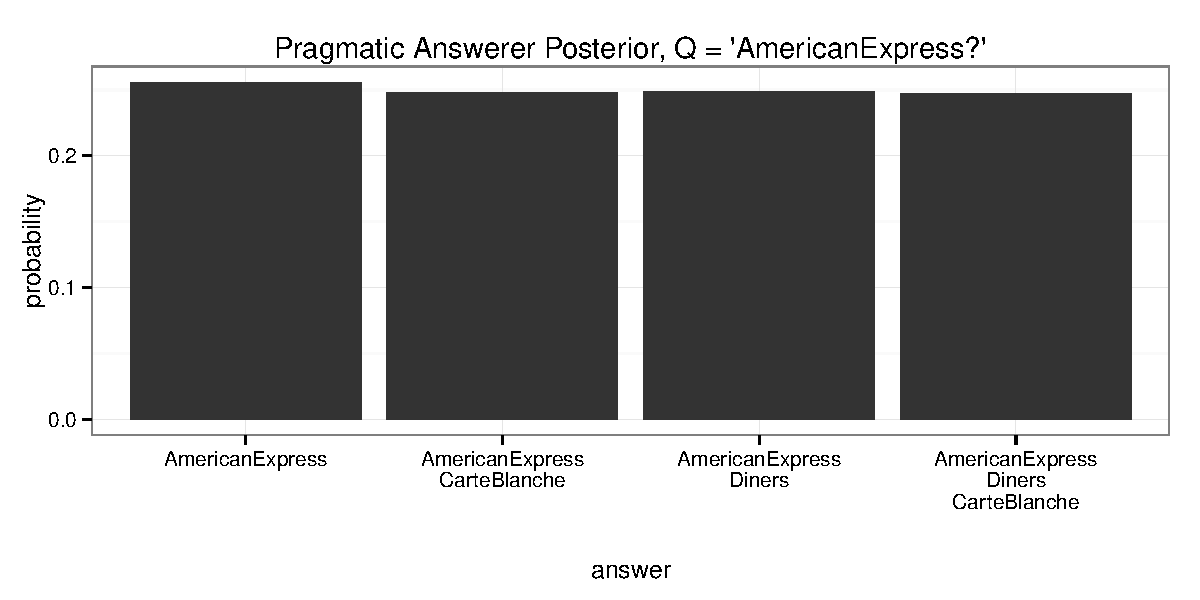
\includegraphics[scale = .6]{americanExpressPosterior.pdf}
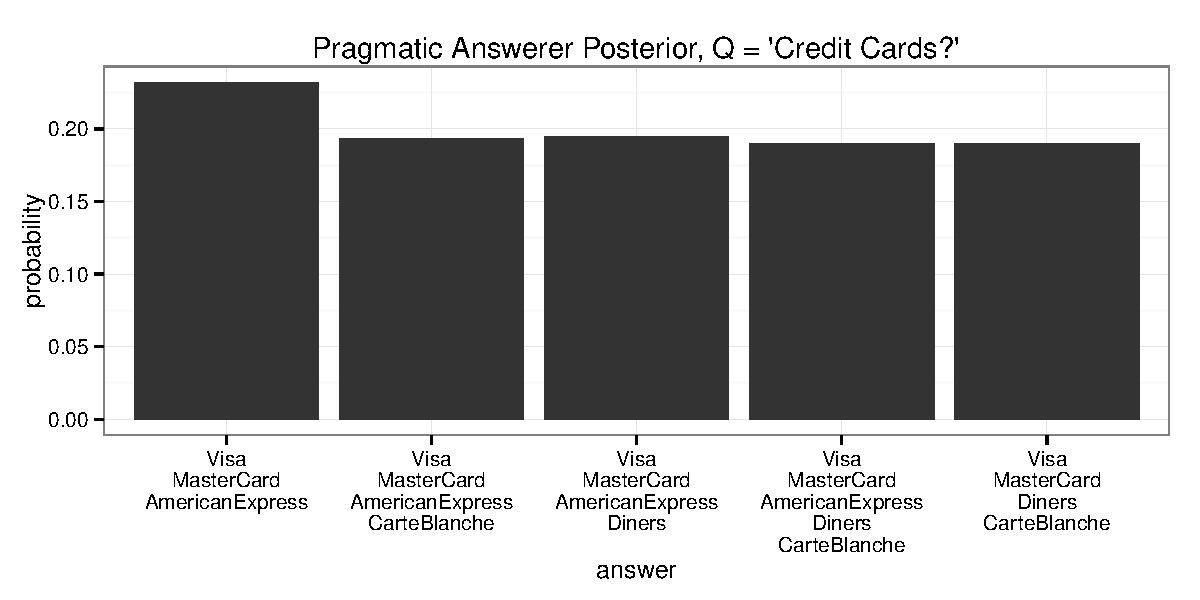
\includegraphics[scale = .6]{creditCardsPosterior.pdf}
\end{center}
\vspace{-.25cm}
\caption{Comparison of questioner goal posteriors that the pragmatic answerer model infers after hearing two different question utterances in Clark (1979), Experiment 5. 
%\todo[inline]{There has to be a better way of presenting this result\dots}
}
\label{fig:clarkExperiment5posteriors}
\end{figure*}

\subsubsection{Results}

We find that when the questioner asks ``Do you accept MasterCard?'', the pragmatic answerer gives a literal ``yes''/``no'' answer with probability $p = 0.92$ (compared to $p=1.00$ empirically). Similarly, when the questioner asks ``Do you accept American Express?'', the pragmatic answerer gives a literal answer with probability $p = 0.96$ (also compared to $p=1.00$ empirically). The small difference between these predicted response probabilities comes from the relative likelihoods of the different cards in the true world. However, when the questioner asks ``Do you accept credit cards?'', the probability of a literal response drops to $p = 0.76$ (compared to $p=0.73$ empirically). Our model output therefore provides a good fit to the original experiment data, both qualitatively and quantitatively.

To further understand \emph{why} our pragmatic answerer model behaves this way, we can examine its inferred posterior over questioner goals for various questions (see Figure \ref{fig:clarkExperiment5posteriors}). The key observation is that questioners who are interested in a longer list of cards are more likely to ask the ``Credit cards?'' question than more specific questions, because knowing whether the shop takes \emph{any} cards (as opposed to no cards) is more informative than knowing whether or not they take a specific one. 

We can see this more clearly by considering two situations. First, consider the explicit questioner who is only interested in an American Express card. Any answer to ``Do you accept American Express?'' would fully resolve their goal (``yes'' would leave certainty over accepting it and ``no'' would leave certainty not accepting it). On the other hand, some answers to ``Do you accept credit cards?'' would not be resolving: if the shop responded ``yes'', the questioner would still have substantial uncertainty over whether the shop takes American Express in particular (for example, the shop could say ``yes'' if they only accepted Visa). A questioner with these interests is thus more likely to ask the first question. 

Now, consider the questioner who is interested in a long list of cards (say, all but Diner's Club). Then getting a yes/no for any one card would fail to address their goals: if they asked ``Do you accept American Express'' and got a ``no'', they are still uncertain wether another of their cards would be accepted. On the other hand, ``Do you accept credit cards?'' is highly informative; if they got a ``no'', they are certain that none of their cards are accepted and if they got a ``yes'', then there is only one possible world where one of their cards won't be accepted (the one where the shop only accepts Diner's Club and no others). A questioner with these interests is thus more likely to ask the second question.

The prediction of the pragmatic answerer model is that the shop will take into account the alternative questions a particular customer \emph{could have} asked but didn't. 

Thus, a pragmatic answerer who hears the question ``Do you accept American Express?'' reasons that the questioner would have asked the other question if they were interested in a long list of cards. Because they didn't ask that question, they must not have been interested in a long list of cards -- just American Express and perhaps a few less common cards (see Figure \ref{fig:clarkExperiment5posteriors}, top panel). The pragmatic answerer is then justified in preferring the resolving ``yes/no'' response; giving an exhaustive list of accepted credit cards is still a \emph{valid} answer, but useful only in a small number of worlds (e.g. where American Express is not accepted but Carte Blanche and/or Diner's card \emph{are} accepted).

Similarly, when asked "Do you accept credit cards?'' the pragmatic answerer reasons that if the questioner were interested in a particular card $c$, they would have asked the more direct question ``Do you accept card $c$?'' and because they did not ask this question, it must not have been the goal. This inference also rules out goals where the questioner has one common card $c$ plus one or more rarer cards, since these goals also lead to the question ``Do you accept card $c$?'' With all these goals ruled out, we are left with five goals in which the caller has \emph{both} common cards (Visa and MasterCard) along with various other less common cards (see Figure \ref{fig:clarkExperiment5posteriors}, bottom panel). The answerer is uncertain as to which set of less common cards are owned. Thus, for any world where the restaurant does not accept Visa or MasterCard, an exhaustive list of accepted cards is determined to be the most informative answer on average. Note that these inferences are made purely on the basis of the questioner model's behavior under possible goals, rather than cues from context as in the previous simulations.

\subsection{Discussion}

In these four case studies, we illustrated several mechanisms our answerer model can use to display sensitivity to questioner goals: answerers may use context, general world knowledge, and most critically, questioner utterances themselves to infer and informatively address the questioner's underlying interests. Additionally, given natural assumptions about priors and sets of alternative questions, answers, and goals, we can use these mechanisms to explain a range of sophisticated psycholinguistic phenomena, both qualitatively and quantitatively.

%One salient issue with our computational experiments is that our resulting answer distribution depends in each case on hard-coded settings such as the space of alternative questions, answers, and goals and the mathematical form of the various priors. We set these components to be simple and natural in the context of the scenario being modeled, but there is still some concern over the amount of flexibility afforded to the modeler in making these choices. For example, the answer prior for both Clark studies uses a parameter to determine the answerer's baseline preference for `yes' and `no' responses versus prices or lists of card types. In both cases we set this parameter to be $p = 0.5$, but other numbers could have been chosen to achieve a better or worse quantitative fit. 

%This raises concerns that our model could fit \emph{any} question-answer data by choosing the appropriate set of priors. Indeed, we regard all of these choices as scientific hypotheses, not free parameters. For the experiments presented later in this paper, we test these hypotheses or fix them via our experiment design. The choices in the computational experiments above were simply intended to be reasonable enough to illustrate how our model framework accommodates various results from the literature on question-answer pragmatics.

Of course, making flexible post-hoc assumptions to capture phenomena inside our computational framework does not, by itself, provide a \emph{test} of our model. The above case studies were intended to showcase the components of the modeling framework and the kinds of explanations it provides, but three additional steps are required to evaluate it. 

First, we must provide empirical evidence for any assumptions we wish to make about priors and alternative spaces for questions, answers, or goals in a particular scenario. Second, we must demonstrate that the \emph{pragmatic} answerer model we emphasized in the case studies above is in fact better than simpler answerer models. Third, while the questioner component of our model was critical to the pragmatic answerer's behavior in the final case study, none of these scenarios tested the predictions of the questioner component or compared the different questioner models against one another. To do so, we need to collect data on which question a questioner prefers to ask given a particular goal. 
  %Our model, following \citeA{VanRooy03_QuestioningDecisionProblems}, however, suggests that the question itself is important in prompting a relevant answer, hence questioner behavior should be treated as a dependent variable.

\section{Guessing Game Experiment: \\Interactive Questions and Answers}

%%%
\begin{figure*}[t!]
\begin{center}
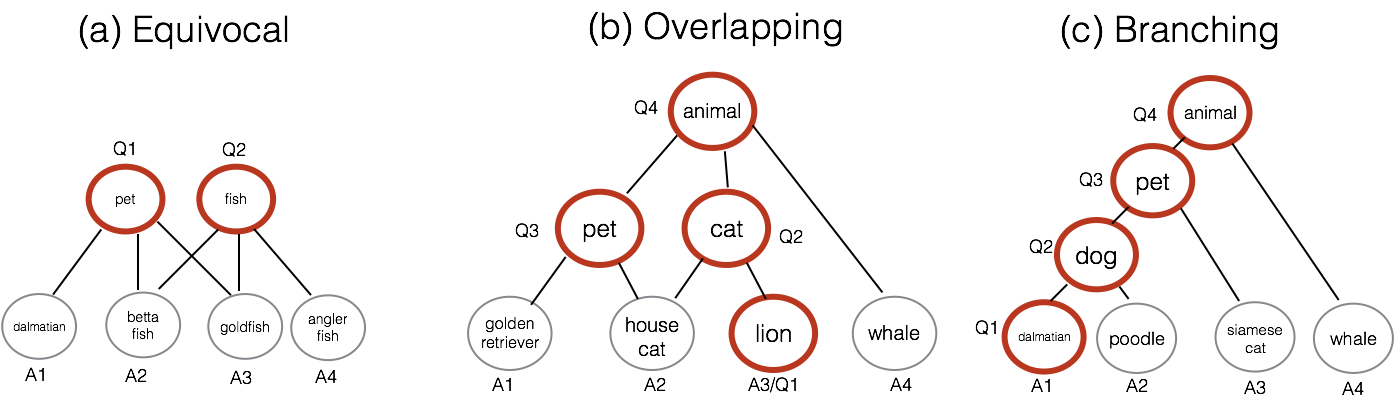
\includegraphics[scale = .3]{hierarchyStructureExamples.png}
\end{center}
\caption{Example of each type of hierarchy. The bottom row served as the answer space, and the labels in the questioner space highlighted in red.}
\label{fig:hierarchyStructures}
\end{figure*}

To satisfy these three requirements, we designed a real-time, multi-player communication game to simultaneously collect data on question-asking behavior \emph{and} answering behavior in an interaction, carefully controlling or measuring priors and alternative spaces. In each round of the Guessing Game task, there are four objects hidden behind four gates such that only one player -- the \emph{answerer} -- knows each object's true location. The other player -- the \emph{questioner} -- is privately assigned one of the objects to find and is allowed to ask one question to query their knowledgeable partner about its location. After hearing the answerer's response, the questioner makes a guess about the location of the target object, then both players receive feedback and advance to the next trial. 

Similar to the Twenty Questions task commonly used in developmental studies \cite{Siegler77_TwentyQuestions, NelsonDivjak___Meder14_GuessWho, RuggeriEtAl15_HierarchicalTwentyQs} this game creates an knowledge asymmetry between players in order to motivate question-asking. Unlike that task, however, we withhold explicit information about the questioner's goal from the answerer. This additional asymmetry, natural to real-world social situations, provides fertile ground for pragmatic reasoning and allows us to test the necessity of goal inference in our models. Critically, both question and answer are selected from restricted sets, such that the alternative set is fixed and in common ground for all participants. In addition to allowing us to avoid ad hoc assumptions about alternative sets when comparing our models, strategic restrictions block the most obvious, direct question and thus allow for richer pragmatic behavior. In this task, we therefore examine \emph{which} indirect question they will use, and how the answerer chooses to respond. 
%These restrictions were motivated by one of the key features of indirect questioning: when the direct question (e.g. ``may I eat your food?'') is suppressed due to politeness, utterance length, complexity, or some other intervening factor, questioners instead rely on a pragmatic indirect question (e.g. ``are you going to eat that?''). 

\begin{figure*}[t!]
\begin{center}
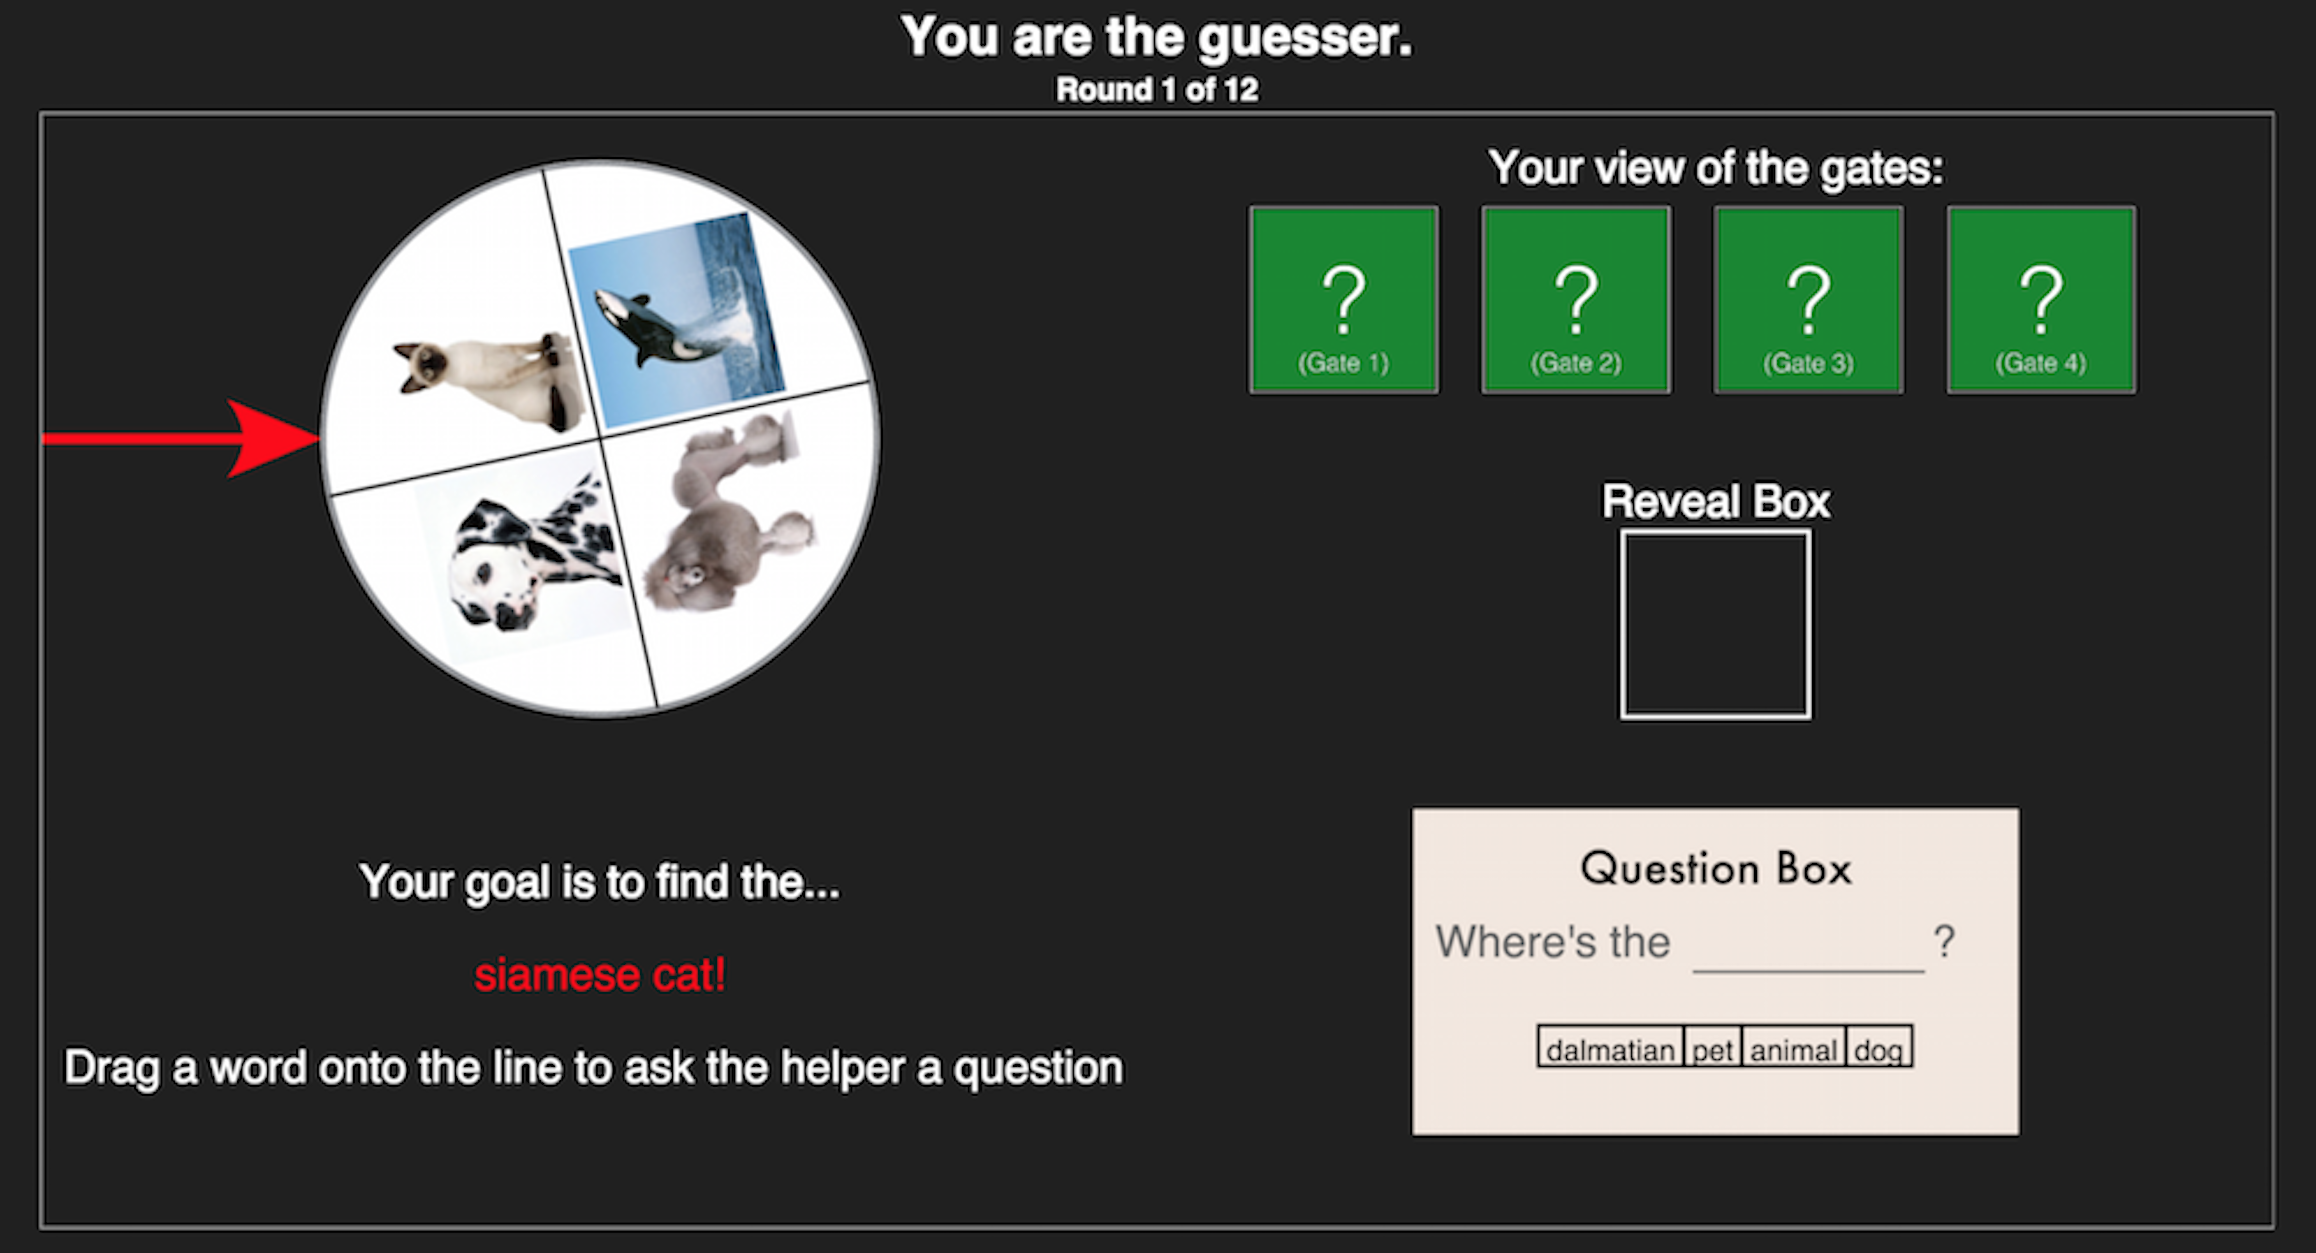
\includegraphics[scale = .213]{Exp4GuesserViewStart}
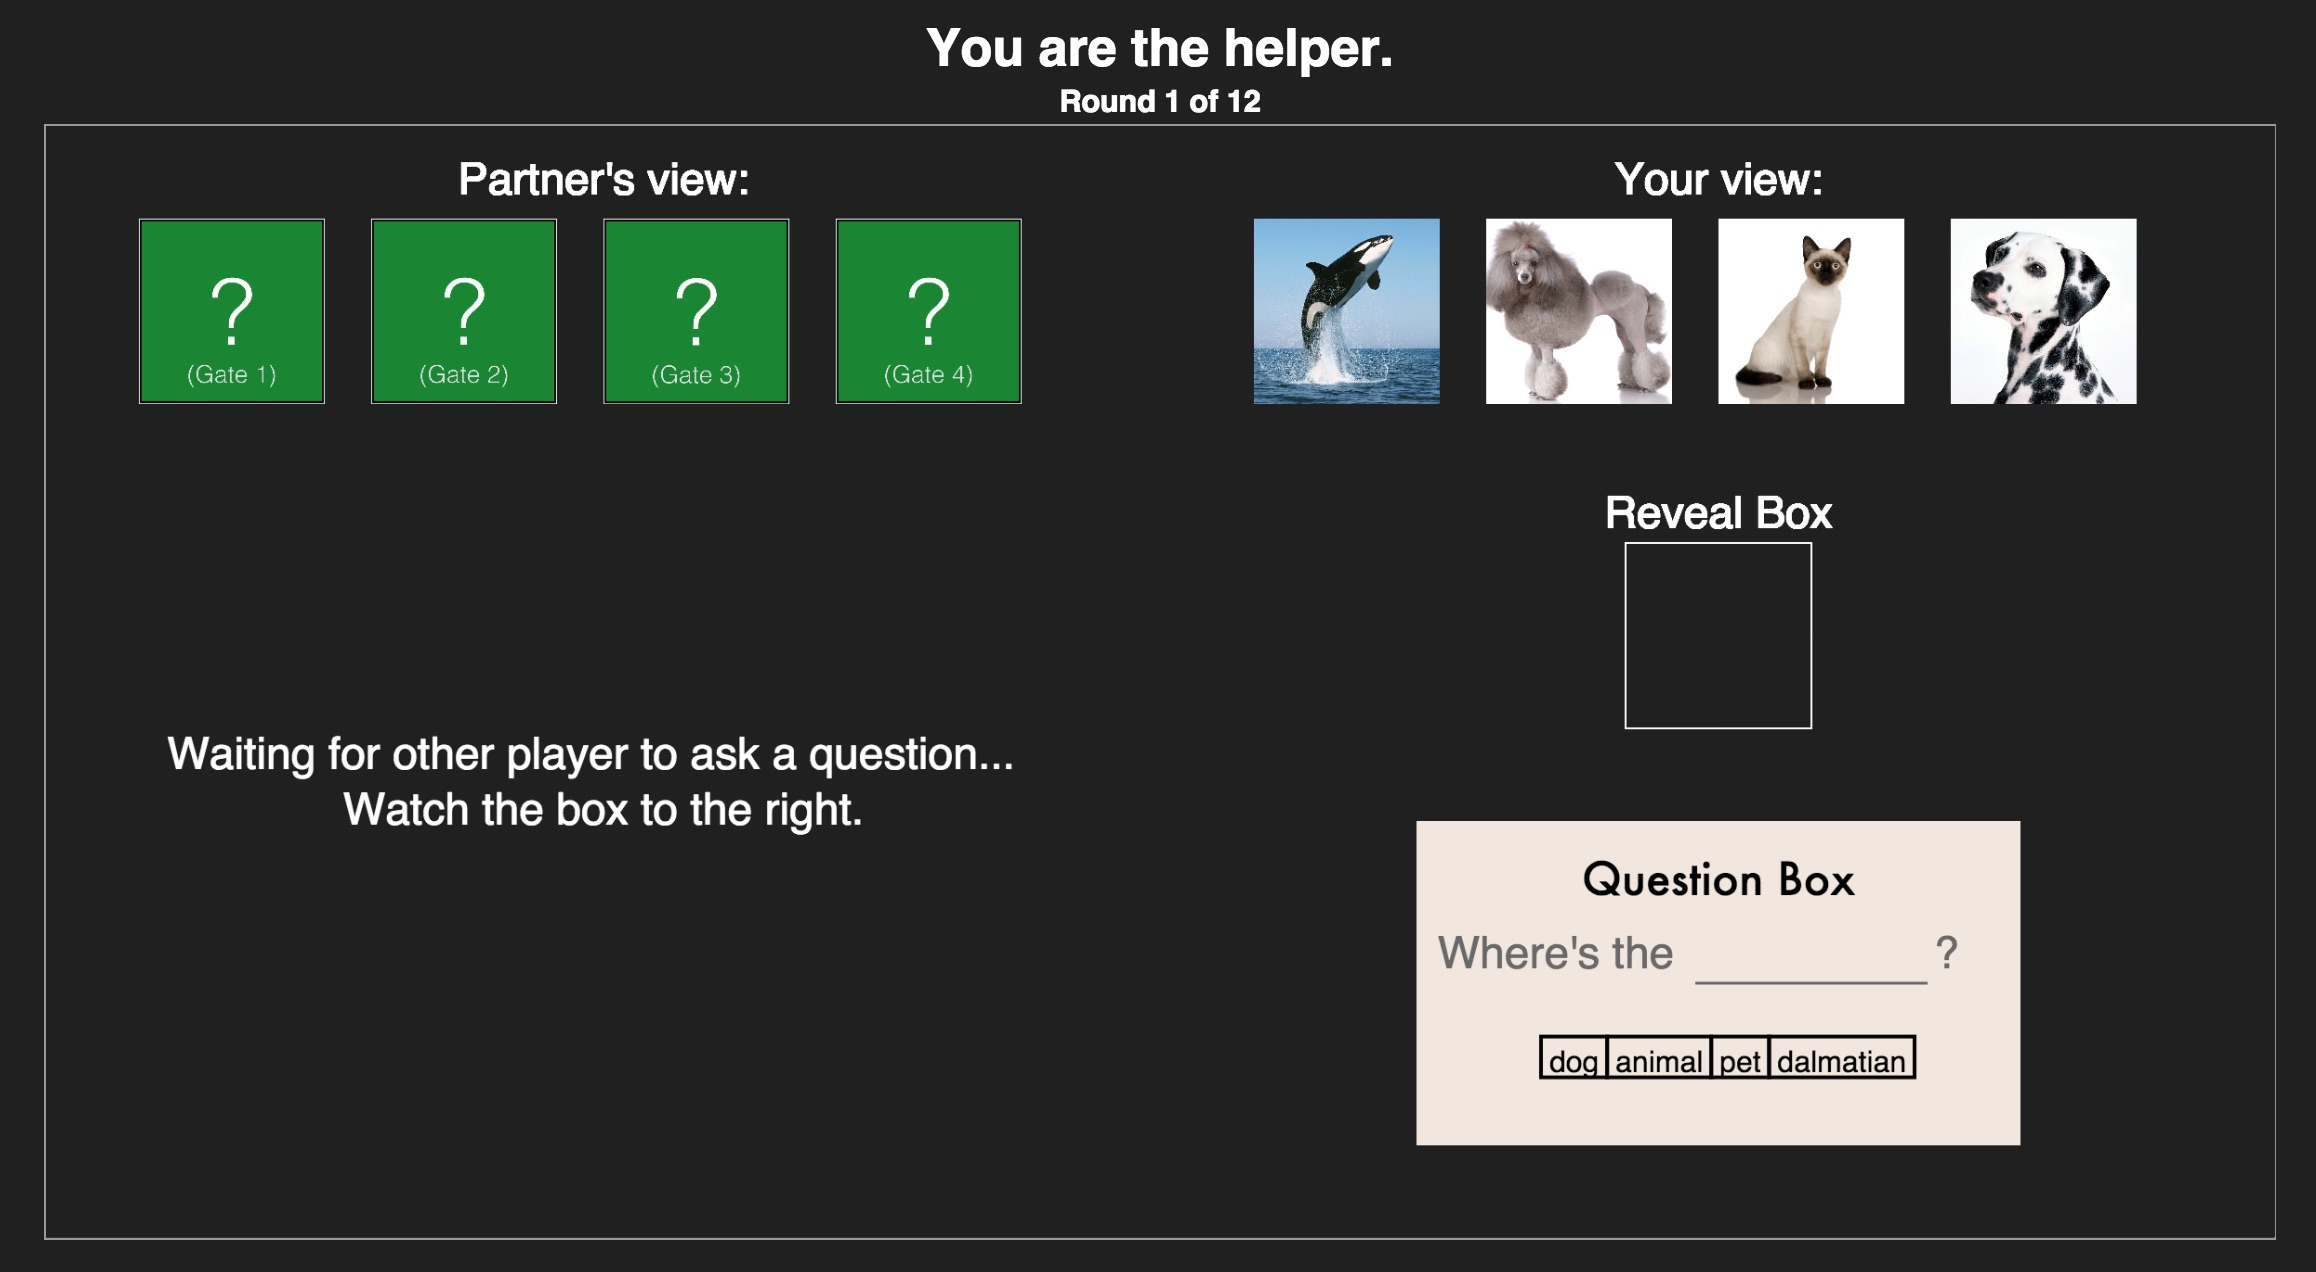
\includegraphics[scale = .105]{Exp4HelperViewStart}
\end{center}
\caption{Experiment interfaces, for the questioner (left) and answerer (right).}
\label{fig:expviews}
\end{figure*}
\subsubsection{Participants} We recruited 199 participants from Amazon's Mechanical Turk to participate in this task. Fifty participants were excluded due to a server crash that terminated the task before completion. Two additional games were excluded because their participants were non-native English speakers. This left 74 unique completed games.

\subsubsection{Stimuli \& Procedure} A set of twelve items were created by crossing four domains (animals, plants, places, and artifacts) with three concept hierarchy structures (``branching'', ``overlapping'', and ``equivocal''; see Figure \ref{fig:hierarchyStructures}) where our models make different predictions. These stimuli exploit the flexibility of our choice of referring expression when referring to objects. A speaker can refer to a Dalmatian as a ``Dalmatian,'' ``dog,'' ``pet,'' or ``animal'' and all would technically be true; . Each item consists of four objects (the leaves of the trees in Figure \ref{fig:hierarchyStructures}) which are hidden behind the four gates and may be assigned to the questioner as goal objects, as well as four question labels drawn from different levels in the concept hierarchy (highlighted in red in Figure \ref{fig:hiearchyStructures}) which the questioner may use to ask about their assigned goal\footnote{A document containing these mappings for all items, as well as their hierarchical relationships, is available online at \scriptsize\url{https://github.com/hawkrobe/Q\_and\_A/stimuliLabels.pdf}}.

The procedure was designed to accommodate real-time player-to-player interaction following \citeA{Hawkins15_RealTimeWebExperiments}. All players passed a short quiz on the game instructions and were immediately redirected to the game interface: the first player to join was assigned to be a ``questioner'' (which we called a ``guesser'' in the cover story) and told to wait until a second player was available. Once another player joined, they were assigned to be an ``answerer'' (or ``helper'') and the game began. 

The questioner and answerer interfaces are displayed in Figure \ref{fig:expviews}. Chat messages were printed on the left side of the screen, and players used the right side as a workspace to view goals, ask questions, and respond with answers. At the beginning of each trial, the wheel on the questioner's screen (Figure \ref{fig:expviews}, top) would spin and select one of the four goals at random. The questioner then clicked and dragged one and only one of the question labels into the pre-set frame ``Where is the\dots?'' to ask a question. The answerer saw these words being dragged in real time. Once the questioner clicked the `send' button, the resulting question appeared in the chat log and control was passed to the answerer, who dragged the objected they wanted to reveal into a ``reveal box.'' The questioner watched as the outline of the gate moved, in real time, and saw the image as soon as the answerer dropped it in the box. Finally, the questioner was asked to click on the gate they believed the goal object was behind. Each participant provided one response for each of the twelve items, presented in random order. 

\subsubsection{Qualitative Behavioral Results}

Before conducting quantitative model comparisons, we highlight several key qualitative patterns in the behavioral data that bear on our theory. First, we note that there was generally high correlation $(r = 0.91 \textrm{ to } 0.97)$ in response probabilities across domains for both questioners and answerers, with the exception of the `place' domain in answerers ($r = 0.78$; see Table \ref{table:experiment4correlations}). We thus collapse across domains in the following qualitative analyses, using labels from the ``animal'' domain for concreteness.

Second, answerer responses deviated significantly from a uniform distribution across true statements. The strongest example of this deviation is in the branching hierarchy. Suppose the questioner asked ``Where is the animal?'' Since all four objects are animals, we might expect an answerer relying solely on the meaning of the utterance to have no preference over which of the animals to provide information about. Our explicit answerer model makes this qualitative prediction. Instead, 94\% of answerers responded with the location of the ``whale,'' the object that isn't described by any of the other questions, $\chi^2(3) = 210.8, p < 0.001$. 

This non-uniform pattern, also found by \citeA{HawkinsStuhlmullerDegen15_qAndA}, is consistent with the Gricean reasoning of our \emph{pragmatic} answerer model: if the questioner was assigned any of the other objects as their goal, they would have been more likely to ask a different question (e.g. if looking for the Dalmatian, they would be more likely to ask ``Where is the Dalmatian?''). Through such counterfactual reasoning, a pragmatic answerer can infer that the questioner's goal is likely to find the whale and respond accordingly. 

Next, we turn to a subtler qualitative pattern in the ``overlapping'' condition (see Fig. \ref{fig:hierarchyStructures}), which was specifically designed to distinguish between our \emph{questioner} models. Suppose the questioner is assigned the ``house cat'' as their goal object. What question do they ask? The explicit questioner model predicts that the two parents -- ``Where is the pet?'' and ``Where is the cat?'' -- should be equally likely, since the explicit answerer they reason about would have a 50\% chance of responding with the house cat's location in either case. 

The \emph{pragmatic} questioner model, on the other hand, predicts that ``cat'' will be preferred over ``pet'', because the other child of ``cat'' -- the lion -- is pragmatically blocked. When the pragmatic answerer hears ``cat,'' they reason that if the questioner's underlying goal were the ``lion'' they would have \emph{said} lion; because they didn't, they must mean the other cat. Thus, we have a pair of sharply distinguishable predictions: the explicit model predicts that ``pet'' and ``cat'' will be equally likely and the pragmatic model predicts an asymmetry where ``cat'' is the preferred label. 

\begin{figure}[t!]
\begin{center}
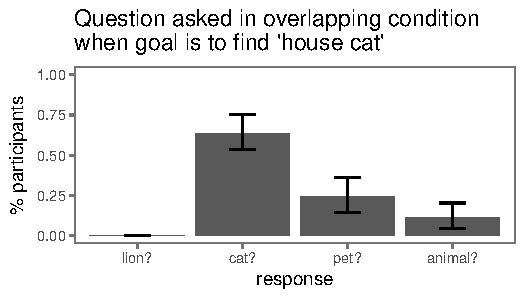
\includegraphics[scale=.46]{OverlappingModelComparison.pdf}
\end{center}
\caption{Questioner responses on overlapping condition. Labels drawn from `animals' domain; probabilities estimated across all domains. Error bars represent bootstrapped 95\% confidence intervals.}
\label{fig:Exp4ZoomedIn}
\end{figure}

The proportion of participants asking each possible question in this scenario, collapsed across domains, is shown in Fig. \ref{fig:Exp4ZoomedIn}. We find that the pragmatic model makes the correct qualitative prediction -- the empirical probability of responding ``cat'' ($\hat{p} = 0.64$) is significantly different from the  probability of responding ``pet'' ($\hat{p} = 0.25$; bootstrapped $95\%$ CI on difference: $[0.17, 0.58]$). This critical condition thus provides evidence that questioners may consider the answerer's inference about likely underlying goals when selecting their question. 

%Thus, in examining the results below we will collapse across domains for simplicity of analysis. 
%Still, it is worth noting that the ``place'' domain has the lowest inter-domain correlations for both questioners and answerers, indicating that it may be an outlier -- we will return to this point in the discussion below.  Next, we step through the response patterns for each hierarchy type. For concreteness, though all statistical tests were conducted on data pooled across domains, we report our results in terms of the `animal' domain instead of the abstract goal, question, and answer labels (see Figure \ref{fig:exp4res} for the full response distributions).
%
%\begin{figure*}[t!]
%\begin{center}
%\includegraphics[scale = .75]{Exp2QuestResults}
%\includegraphics[scale = .75]{Exp2AnsResults}
%\end{center}
%\caption{Results and model fits, for the best-performing questioner (left) and answerer (right) models, collapsing over the different domains. Error bars represent bootstrapped 95\% confidence intervals.\todo[inline]{Judith: axes difficult to read. Maybe just use animal labels here? Or move to supplemental?}}
%\label{fig:exp4res}
%\end{figure*}

%In the `overlapping' condition (Figure \ref{fig:hierarchyStructures}(b)), questioners preferentially asked about the `lion' when looking for the lion, $\chi^2(3) = 205, p < 0.001$; about the `cat' when looking for the Siamese cat, $\chi^2(3) = 63, p < 0.001$, even though the lion is also a cat; about the `pet' when looking for the dalmatian, $\chi^2(3) = 232, p < 0.001$, even though the Siamese cat is also a pet; and about the `animal' when looking for the whale, $\chi^2(3) = 213, p < 0.001$. Answerers preferentially revealed the lion when asked about the `lion,' $\chi^2(3) = 229, p < 0.001$, the Siamese cat when asked about the `cat,' $\chi^2(3) = 59, p < 0.001$, the dalmatian when asked about the `pet,' $\chi^2(3) = 120, p < 0.001$, and the whale when asked about the `animal,' $\chi^2(3) = 187, p < 0.001$. 

%In the `branching' hierarchy (Figure \ref{fig:hierarchyStructures}(c)), we found that questioners strongly prefer to ask about the `dalmatian' when trying to find the dalmatian, $\chi^2(3) = 190, p < 0.001$, about the `dog' when trying to find the poodle, $\chi^2(3) = 152, p < 0.001$, about the `pet' when trying to find the siamese cat, $\chi^2(3) = 168, p < 0.001$, and about the `animal' when trying to find the whale, $\chi^2(3) = 210, p < 0.001$. %Answerers respond in kind. , and in an earlier version of the multi-player study we report in this section.

\subsubsection{Model comparison}

These results show that our non-pragmatic models cannot account for key qualitative phenomena while our pragmatic models make the correct predictions. Next, we show that our pragmatic models also provide better overall quantitative fits to the behavioral data. Before showing the results of our direct model comparison, we formalize the experimental task in our modeling framework. 

Corresponding to the structure of our experiment design, we take the set of possible worlds $\mathcal{W}$ on a given trial to be the set of possible permutations of the four objects to the four locations (yielding $4! = 24$ possibilities). Because we explicitly instructed questioners to be find the location of a particular object, we then take the space of goals $\mathcal{G}$ to be the set of goal projections $$g_o(w) = \textrm{loc}(o,w)$$ where $\textrm{loc(o,w)}$ is a simple function looking up the location of object $o$ in world $w$. 

To populate our question space $\mathcal{Q}$, we must specify the explicit meaning of the question ``Where is the $x$?'' for each of the four labels allowed in a given trial (see Fig. \ref{fig:hierarchyStructures}). As in our discussion of \citeA{GroenendijkStokhof84_SemanticsOfQuestions} above, we take \textrm{\den{Where is $o$?}} for a given object $o$ to be a projection from a world to the location of $o$ in that world. We then enrich this meaning to account for the use of the definite article \emph{the} for labels at higher levels of the taxonomy (e.g. asking ``Where is the dog?'' when there is more than one dog). Under the standard formal semantics of \emph{the}, the denotation of a noun phrase containing a definite article is only defined if there is a unique, salient object that the noun picks out in the world; pragmatically, then, the use of a definite article \emph{presupposes} the uniqueness or salience of some object in shared context \cite{Lewis79_Scorekeeping, clark1983common, Roberts03_UniquenessDefiniteNounPhrases}. Thus our explicit meaning of each question $q$ is: 
$$\textrm{\den{Where is the x?}} = q_{x}(w) = \textrm{loc}(s_x,w)$$ where $s_x$ is the \emph{salient} object of category $x$. 

Because the answerer does not know \emph{a priori} which object is the salient one, they interpret the question by drawing an object from a saliency distribution, given the category in the noun phrase: $s_x \sim \mathcal{S}(o | x)$. This distribution may depend on typicality judgements \cite{Rosch75}, world knowledge about what labels people tend to use to refer to different objects, and so on. For this section, we take the saliency prior to be uniform over all objects that are within a category (e.g. over all leaves of the subtree beneath the given label; see Fig. \ref{fig:hierarchyStructures}). Finally, the answer space $\mathcal{A}$ is the set of constructions ``The $o$ is behind gate $i$.'' which evaluate to true in worlds where $o$ is at location $i$ and false otherwise.  %\footnote{Later, we will collect empirical saliency priors, and show how this affects the model's fit.} Note that other variations of the question, such as ``Where \emph{are} the animal\emph{s}?'', would be given different semantics (e.g. projecting a world to the set of all locations occupied by animals rather than the single location of the salient animal). 

For a rigorous model comparison among explicit and pragmatic models, we conducted a Bayesian data analysis \cite{LeeWagenmakers14_BDA}. For our data analysis, we introduce a binary parameter $\gamma \in \{\textrm{explicit}, \textrm{pragmatic}\}$  determining which model's likelihood function to use, and jointly infer this parameter along with a rationality parameter $\alpha$ for each model by conditioning on our empirical data. After integrating over values of $\alpha$, the posterior $P(\gamma | \textrm{data})$ can be interpreted as the relative evidence for each model \cite{KruschkeVanPaemel15_OxfordHandbook}, from which a Bayes Factor can be computed:

$$BF = \frac{P(\textrm{data}\, |\, \gamma = \textrm{pragmatic})}{P(\textrm{data}\, |\, \gamma = \textrm{explicit})}$$

We place uninformative priors over these parameters $$\gamma \sim Bernoulli(.5)$$ $$\alpha \sim Unif(0,20)$$ and perform inference using enumeration over discrete bins. This gives us a 

 Each model was run with uniform prior probability over worlds, goals, questions, and answers, and with equal cost for all utterances. 


\begin{figure*}[t!]
\begin{center}
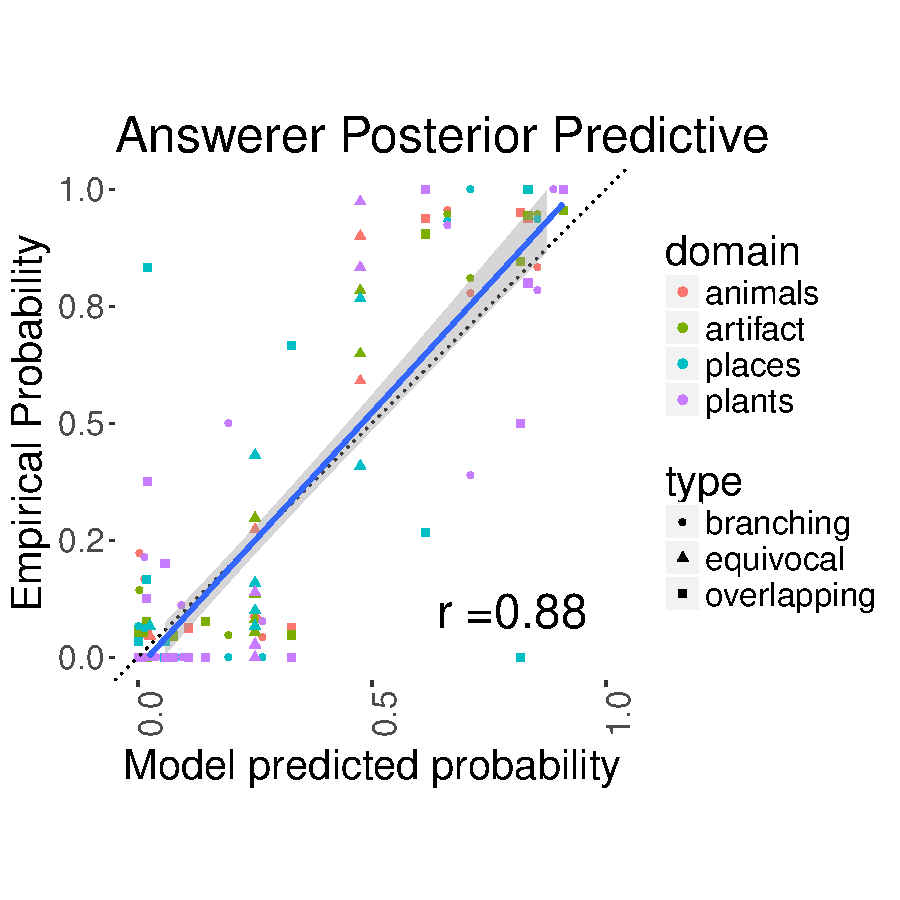
\includegraphics[scale=.5]{betaZeroAnswerer_Predictives}
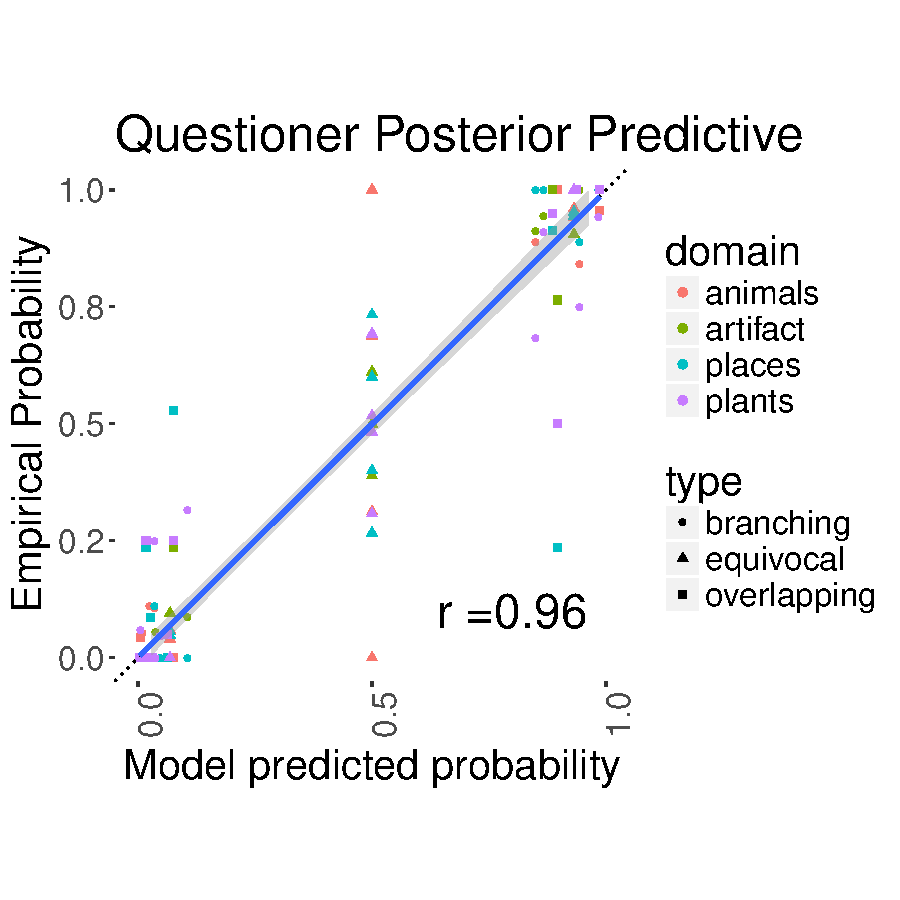
\includegraphics[scale=.5]{betaZeroQuestioner_Predictives}
\end{center}
\caption{Full space of models, and their correlations with the data, broken down by item and type.}
\label{fig:Exp2ModelSpace}
\end{figure*}


%

%

%\todo[inline]{TODO: replace these correlations with a BDA \& predictives plot}

%These model-data fits are displayed in Figure \ref{fig:Exp2ModelSpace}. We can immediately rule out the literal answerer and literal questioner, which predict a uniform distribution of responses within each condition. We also find that the pragmatic answerer model ($\alpha = 9.6$) fits the data significantly better than the explicit answerer model ($\alpha = 1.1$), with $r = 0.88$ compared with $r = 0.65$ (Zou's 95\% confidence interval $= [0.16, 0.32]$).  Turning to the questioner predictions, we again find that both explicit ($\alpha = 9.9$) and pragmatic ($\alpha = 6.2$) models provide excellent but essentially indistinguishable fits, with $r = 0.953$ compared with $0.956$ (Zou's 95\% confidence interval $= [-0.02, 0.01]$). 

%We also see that it makes a relatively good quantitative prediction, with the predicted probability lying within the 95\% confidence interval of the empirical estimate for both the ``Q2'' and ``Q3'' responses. 
%Recall that a single free parameter $\alpha$ for each model was fit to maximize correlations for the entire (pooled) dataset. 

\subsubsection{Discussion}

%%We also identified four shortcomings of Experiment 1. First, despite the success in distinguishing between answerer models, our data are not sufficient to distinguish between the explicit and pragmatic \emph{questioner} models. The two models did not make significantly different predictions for this experiment (and both are sufficient to account for the data). 
%
%
%
%Finally, because there was overwhelming agreement among participants on the appropriate question to ask and the appropriate answer to give, our response probabilities are clumped at the ends of the scale. Thus, while there is an excellent quantitative fit between our model and the data, assessed with the correlation coefficient, we were essentially fitting endpoints. We would like to collect more graded judgements between these endpoints, where our model predicts that participants will disagree.
% 

This experiment tested our model in two novel ways. First, we found that only the pragmatic answerer can account for essential qualitative features of the response data. For example, the explicit answerer predicts a uniform distribution over responses to the `animal?' question in the branching hierarchy. All four of the objects are animals and under the assumption that all four are equally salient, the question meaning projection is equally likely to pick out any of them. Contrary to these predictions, we found that answerers overwhelmingly preferred the response ``whale'' to the other three responses, which is accurately predicted by the Gricean dynamics of the pragmatic model. If the questioner were interested in any animal other than the whale, they would have asked a different question; since they didn't, they must have meant the whale. Like our final case study, this task required the answerer to use the questioner's utterance as a signal of their underlying goals -- a more complex scenario than the first three case studies, and one that exercises the full range of our answerer model. 

Additionally, we were able to test the predictions of the \emph{questioner} component of the model for the first time, since questioner responses have not previously been treated as a dependent variable worthy of explanation. We found that at an aggregate level, both the explicit and pragmatic questioner models do a good job of predicting what questions an agent will pick when faced with a particular goal and particular beliefs about how the answerer will reason about their utterance. However, our results for the overlapping hierarchy in particular show that the pragmatic model is necessary to account for some critical aspects of the data. 

The ``place'' domain that we flagged as a potential outlier earlier in the results is the only domain that does not show the pattern of responses predicted by the pragmatic questioner model. This is likely due to the choice of images displayed to participants: the two ``parent'' nodes of the critical goal are ``bar'' and ``restaurant,'' and we represented the intersection of these two categories as a hotel lobby. However, the image we chose placed emphasis in the bar in the hotel, which likely biased participants toward the ``bar'' response instead of the ``restaurant response'' predicted by the pragmatic model. Including it does not change the statistical results, but we do not believe it is representative of questioner behavior. 

\section{Enriching question semantics with saliency knowledge}

While our pragmatic models make the correct qualitative predictions, they clearly fail to capture graded responses across different domains. This is especially striking in the `equivocal' condition where our models predict no preference in questioner behavior: if asking about the goldfish, which is both a ``pet'' and a ``fish,'' the symmetry of the alternatives provides no pragmatic reason to favor one label over the other. Instead, we found a high degree of variability across domains. For example, when questioners were trying to find a pet goldfish, 85\% of participants preferred the label `fish' to the label `pet,' even though both are technically true. In the `artifacts' domain, on the other hand, questioners had no preference between asking about the `seat' or `metal thing' when the objects (metal chairs) fell into both categories.%To some extent, this is expected from a model with only a single parameter fit for all domains simultaneously. We could have fit separate rationality parameters for each domain to capture domain-level differences. However, we expect that this variability can be accounted for in a more principled way by the saliency prior. Our assumption of uniformity may be incorrect. Indeed, we found that 

This could be explained as a typicality effect. A Dalmatian is a far more typical and salient member of the `pet' category than a goldfish \cite{Rosch75}, hence a questioner considering this knowledge as common ground would know that asking ``Where is the pet?'' would tend to elicit information about the dalmatian. If they were looking for information about the goldfish, they would then prefer to ask about the `fish' category, where a goldfish is a highly typical example. 

Typicality effects could also potentially be driving the divergence from a uniform response distribution in the overlapping condition, which we took to be evidence of pragmatic questioner behavior. For example, we expect a house cat to be a much more typical exemplar of the category `cat' than a lion. Hence, participants may not be choosing the house cat in this item for pragmatic reasons; they may just be selecting the more salient member of the category. If this were the case, including saliency knowledge in our explicit questioner and answerer model should give rise to the same predictions as the pragmatic models and `explain away' the pragmatic effects. Finally, we made certain assumptions in modeling our hierarchies, such as the assumption that participants do not consider whales to be pets despite the fact that it's technically possible. 

In this section, we address these issues by collecting data about participants' saliency knowledge. We then recompute our model's predictions using empirical saliency priors as common ground, in  place of our previous assumption of uniform saliency within a category. We conduct a Bayesian data analysis using these new predictions to test (1) whether our models more appropriately capture item-level variability and (2) whether the pragmatic model still provides a better fit after controlling for typicality knowledge.

\subsection{Participants} 
We recruited 192 participants from Amazon's Mechanical Turk to participate in this task. 13 participants were excluded after reporting a non-English native language, and 15 more were excluded due to self-reported confusion over the instructions. This left data for 164 participants.

\subsection{Stimuli \& Procedure}
For each trial, participants were presented with a set of four pictures and asked to ``Click the $X$,'' with $X$ being some label that might refer to multiple pictures. Each participant provided a response for twelve trials, corresponding to the twelve items from our experiment above (three hierarchy structures crossed with four domains). The four pictures corresponded to the four goal objects of the given item; we used the same pictures that were displayed on the questioner's goal wheel and the answerer's `gates.' The instruction ``Click the $X$'' for a given set of pictures was formed by sampling one of the four category nouns that could be used to form a question (the highlighted nodes in Fig. \ref{fig:hierarchyStructures}). In this way, no participant saw the same set of objects more than once (although some images occurred in multiple sets). The order of trials and positions of pictures within trials were randomized.

\subsection{Results}

For each label, we computed the proportion of participants that clicked on each of the objects, forming a saliency distribution $s_N \sim \mathcal{S}(o | N)$. To test the null hypothesis of uniform saliency distribution we assumed in the foregoing model comparison, we performed $\chi^2$ goodness of fit tests on the response distribution for each label: a total of 32 tests. We found that 69\% of these tests rejected the null hypothesis of uniformity at a (Bonferroni-corrected) significance level of $\alpha = 0.05/32 = 0.002$ indicating that our initial assumption was not justified. 

We next carried out a model comparison using these empirically measured saliency distributions instead of assuming uniform. We find that the pragmatic answerer model provides a significantly better fit to the data than the explicit model, with $r=0.91$, compared to $0.72$ (Zou's 95\% confidence interval $= [0.13, 0.27]$). The pragmatic questioner model also provides a slightly better fit to the data than the explicit model, with $r = 0.92$ compared to $0.89$ (Zou's 95\% confidence interval $= [0.01, 0.06]$). 

For a more precise test of whether participants are using uniform priors or the distributions we measured empirically, we conducted a Bayesian data analysis of our questioner and answerer models \cite{HemmerTauberSteyvers15_BDAplus}. For the purposes of this analysis, we model the saliency prior as a mixture of the uniform distribution assumed in earlier experiments and the saliency distribution we empirically measured. 

\begin{figure}[th!]
\begin{center}
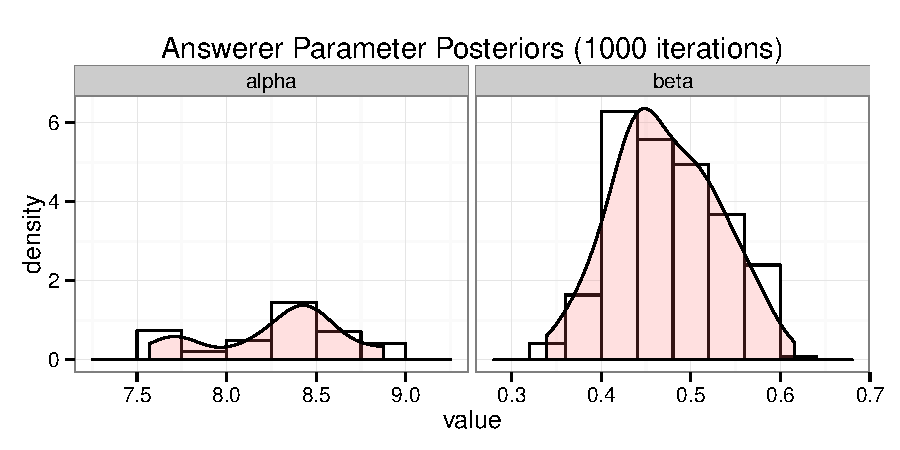
\includegraphics[scale=.5]{AnswererParamPosteriors.pdf}
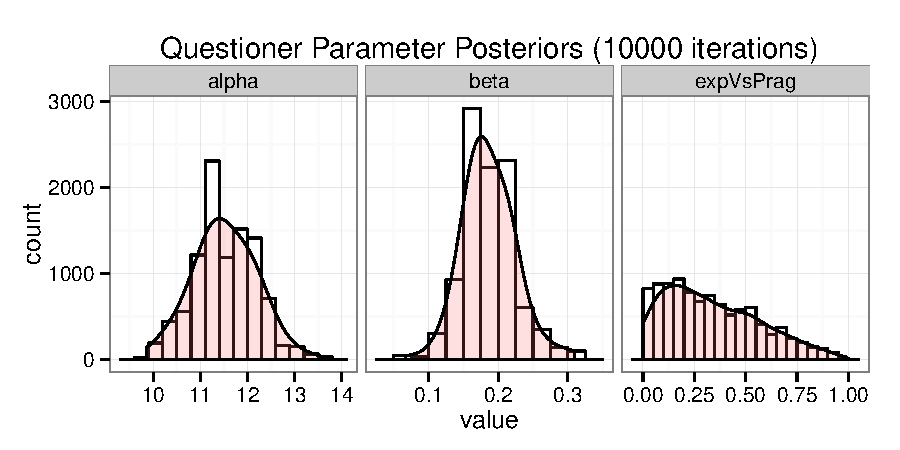
\includegraphics[scale=.5]{QuestionerParamPosteriors.pdf}
\end{center}
\caption{Posteriors for the parameters inferred by our Bayesian data analyses. 
%\todo[inline]{Label questioner row; include (dumb) bar plot of gamma on log scale?}
}
\label{fig:BayesianParamPosteriors}
\end{figure}
\subsection{Discussion}

We introduce a parameter $\beta \in [0,1]$ controlling the mixture weight, with $\beta = 0$ corresponding to a pure uniform distribution and $\beta = 1$ corresponding to a pure empirical distribution. 

\begin{figure*}[t!]
\begin{center}
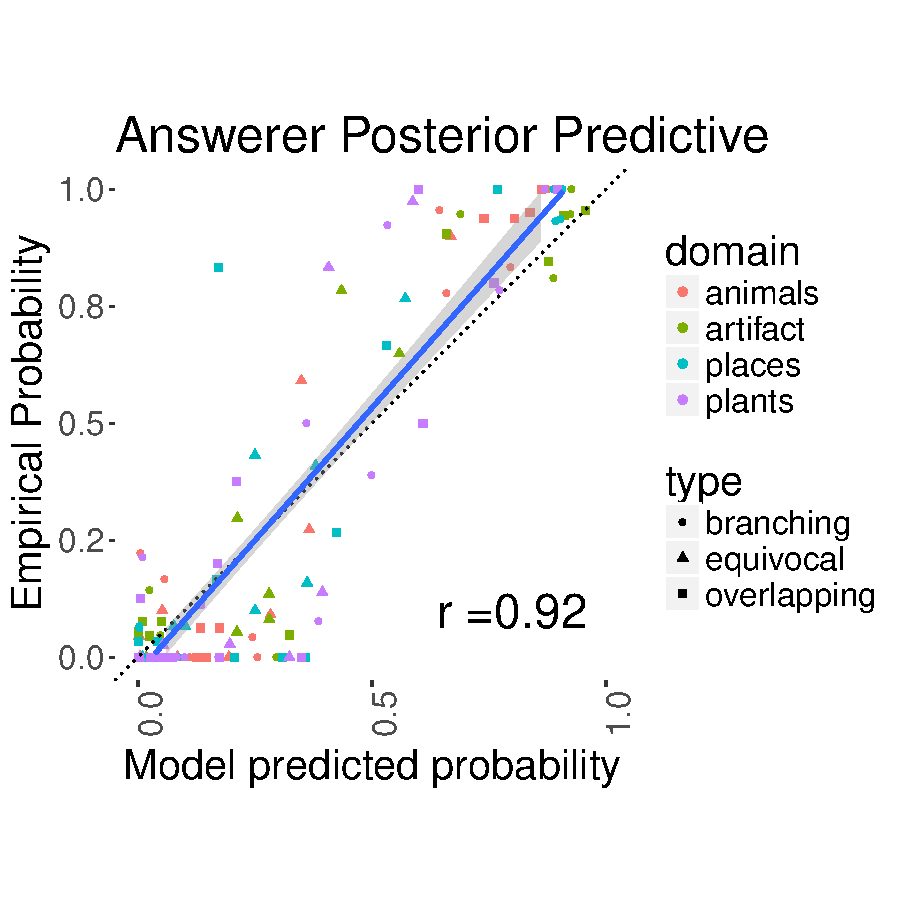
\includegraphics[scale=.5]{fullAnswerer_Predictives}
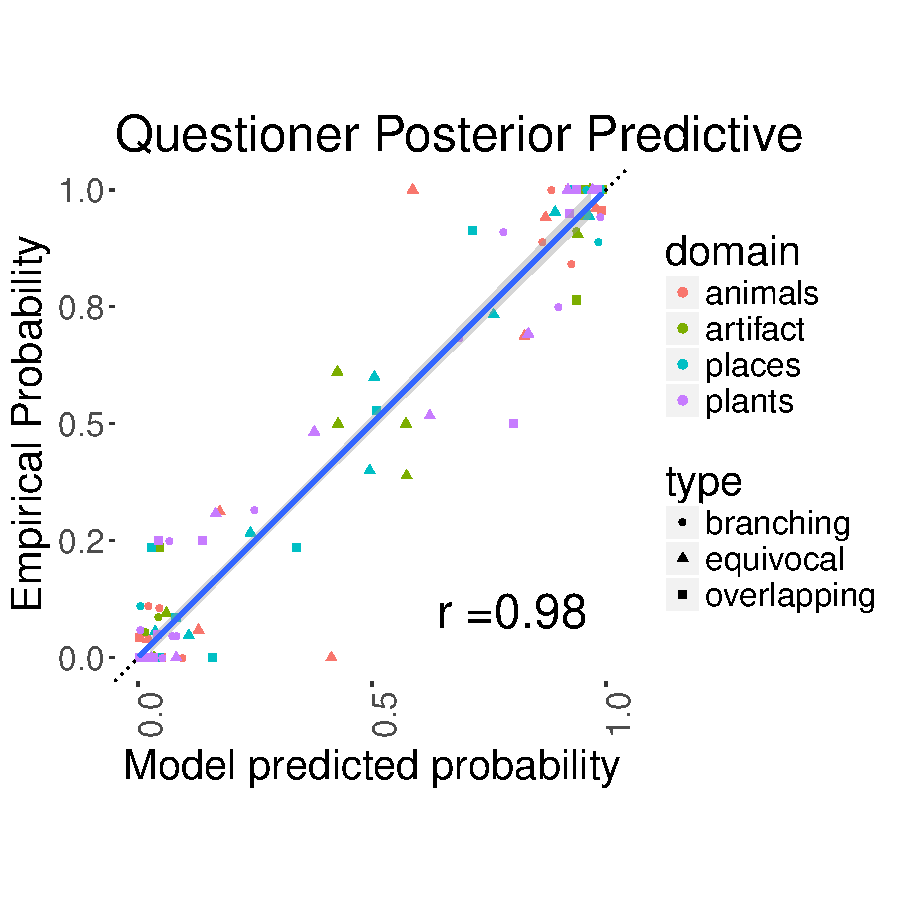
\includegraphics[scale=.5]{fullQuestioner_Predictives}
\end{center}
\caption{Model-data fit for posterior predictives. Vertical error bars are bootstrapped 95\% confidence intervals for estimated probabilities. Horizontal error bars are 95\% highest posterior density intervals around the MAP estimate.}
\label{fig:posteriorPredictives}
\end{figure*}

We first note that the posterior distribution of alpha values inferred here roughly match the maximizing alpha values found by grid search in earlier experiments, with a modal value of $\alpha = 8.05$ (95\% highest posterior density (HPD) interval $=[7.3, 8.7])$ for the answerer model and $\alpha = 6.25$ (95\% HPD $=[6, 6.5]$) for the questioner model. Second, we found maximum a posteriori (MAP) beta values of $\beta = 0.5$ (95\% HPD $=[.4, .55]$) for our answerer model, and $\beta = 0.35$ (95\% HPD interval $= [0.3, 0.45]$) for our questioner model, implying that both questioners and answerers use a mixture between a purely uniform and purely empirical saliency prior. Finally, our model comparison parameter $\gamma$ showed overwhelming evidence for the pragmatic answerer model (BF $= \sim6 \times 10^{72}$) and strong evidence for the pragmatic questioner model (BF $= \sim2\times 10^{7}$).

Our Bayesian data analysis resolves several concerns about our previous results. We found that the dominance of our pragmatic answerer model over the explicit answerer model could not be explained by saliency or typicality: after incorporating saliency priors into the model, the pragmatic answerer model still accounted for response data much better than the explicit answerer model. In fact, we found that participants used a slightly flattened version of the empirically measured saliency prior. This mixture may be partially due to the fact that our saliency prior elicitation task still inevitably introduces pragmatic demands. When a participant is instructed to ``Click the $X$,'' they may think about the alternatives and which one the experimenter would be referring to as the most salient. Thus, our empirical saliency prior might be stronger than the true prior. While this does not pose a problem for our purposes, we suspect that one may be able to tease out the true prior by modeling the saliency elicitation task and conducting a further Bayesian data analysis.

Additionally, despite difficulties distinguishing between the explicit and pragmatic questioner models by comparing correlations with data in previous experiments, our Bayesian data analysis allowed us to conduct a stronger and more direct model comparison. We found that strong evidence that questioners consider pragmatic answerers when selecting a question to ask. Even at its MAP parameter values, the explicit questioner could not account for responses in the `overlapping' condition we designed to distinguish the two models. Finally, by examining the posterior predictive, we found that by incorporating a mixture of uniform and empirical saliency priors, we were able to capture item-level variability much more comprehensively than in previous experiments. 

\section{General discussion}
\label{sec:gd}

%\todo[inline]{Might split this into subsections?}
% \subsection{Summary of what we did}

Asking questions is one of our most efficient and reliable means of learning about the world. This method of social learning, however, depends crucially on the questioner's ability to choose a ``good'' question and the answerer's ability to give a ``good'' answer. In this paper, we presented a quantitative model specifying a theory of exactly what constitutes a ``good'' question or answer. Specifically, we argue that at a computational level, questioner and answer choices are determined through recursive social reasoning. Questioners consider likely answers and seek to maximize the reduction in their own uncertainty. Answerers, in turn, seek to informatively address the questioner goals most likely to have generated the question. We provided several lines of evidence for this theory. 

%\todo[inline]{Refactor next paragraph to separate out stuff that's included in the model from external stuff}
First, in four case studies, we showed how this modeling framework explains classic results about answerer sensitivity to context and questioner intentions. These computational experiments highlighted several mechanisms that answerers can use to adjust their responses. Elements of the context, like the questioner's previous utterances, and general world knowledge, like the increasing likelihood of being in a hurry closer to a meeting, can shift the answerer's prior about the questioner's likely goals. In many scenarios, the questioner utterance itself is informative about underlying goals. 


Second, in a real-time, multi-player experiment, we found additional evidence for answerer sensitivity to questioner goals based on the questioner utterance. In a series of model comparisons, we showed that answerer behavior is best described by a pragmatic model that reasons about underlying questioner intentions. %The superiority of pragmatic answerer predictions over the other answerer models was robust across all experiments and conditions, and it provided an excellent fit to the data in an absolute sense despite having very few free parameters.

Third, by manipulating questioner goals in these two experiments, we observed systematic use of indirect questions. Our questioner models, especially when enriched by empirical saliency priors, provided an excellent fit in a range of different scenarios. We found that at least in certain critical scenarios like the overlapping hierarchy condition of Exp~.2, questioners relied on higher-order pragmatic reasoning about what inferences an answerer would make about their own underlying goals when deciding what question to ask, but a Bayesian model comparison showed that the simpler explicit model is sufficient to explain the vast majority of our data.

%In the case of our Experiment 1 hierarchy, there exists a simple, heuristic strategy that produces the same pattern of responses as our model without requiring any social inference. Suppose questioners saw their goal on a given trial and ruled out labels that do not apply (e.g. a `cat' is neither a `dalmatian' nor a `dog'), then picked the most specific of the remaining labels (`pet' picks out a smaller set of objects than `animal'). Whether through use of this heuristic strategy or pragmatic inference (as our model suggests), questioners strongly converged on a single mapping from goals to question utterances. 

 Note that this behavior also could not be explained by the heuristic strategy raised in the earlier experiments: if questioners just ruled out labels that did not apply (e.g. ``lion''), they would have no mechanism for deciding between the two equally-good parent labels (``pet'' and ``cat'') to pick out their goal. 

Perhaps the most important formal advance of the models considered here is to move the Rational Speech Act framework beyond interpretation of single utterances (in context), to consider the dynamics of simple dialogs (albeit consisting of a single question and its answer). 
Doing so requires replacing the immediate motive to convey true information with the more distant motive to provoke useful information from one's interlocutor. On the answerer side, sophisticated inference was required to account for the implicit interests of the questioner. This provides a useful connection to current game-theoretic and decision-theoretic models \cite{VogelBodoiaPottsJurafsky13_GricePOMDP, VanRooy03_QuestioningDecisionProblems}, which also emphasize the importance of goals and speaker beliefs in communication but emphasize less the complex interplay of inference between questioner and answerer.

% Questioner behavior, however, appeared to be more sensitive to the experimental set-up. In a single-player pilot version of Exp.~1, for example, we did not emphasize certain aspects of the game in the instructions, such as the fact that the answerer knows about the restricted answer set. Our data in this pilot experiment appeared to contain a mixture of explicit and pragmatic answerers and questioners (though other confounds were present in this version). We found the interactive, multi-player version of the task, used in this paper to be more robust to these minor variations. 

%\subsection{Limitations of the model}

We emphasize that all our models are situated firmly at the computational level \cite{Marr10_Vision} -- these models formalize hypotheses about the problem being solved by questioners and answerers in dialogue, and they make quantitative predictions about expected behavior under different assumptions. However, we do not propose that people are actively running a recursive probability calculation online every time they ask a question; further work is needed at the algorithmic and mechanistic levels to understand exactly what cognitive and neural processes give rise to the computations we predict, especially when it comes to integrating information across discourse contexts. 

While these results provide strong evidence for our claim that question-asking and answering is grounded in sophisticated social reasoning, it is worth more closely examining some choices we made in formulating our Rational Speech Act model. For example, as in previous studies using RSA, we assume that the recursive reasoning process giving rise to pragmatic interpretations grounds out in a base case of literal semantics. We only consider two levels of recursion above this base case, but we could in principle consider a fixed-point at infinity \cite{Franke13_GameTheoryPragmatics}. Alternatively, social reasoning could be grounded not in iterated reasoning but in a joint project or shared intention established by other means \cite{Clark96_UsingLanguage, TomaselloCarpenter___Moll05_IntentionsCulturalCognition}. While we suspect the question-answer domain is not particularly informative for distinguishing between these formulations, we note that additional levels of reasoning tend not to qualitatively change RSA predictions and that our model contains elements of the latter proposal in its assumption that questioners and answerers share priors, sets of alternatives, and semantic meanings in common ground \cite<see>[for further discussion]{LassiterGoodman15_AdjectivalVagueness} 

It is also unclear whether our notion of goals as projections is sufficient to capture the semantics of all kinds of questions, and whether our assumptions scale up to less constrained interactions. In social scenarios with strongly conventionalized or constrained schemas, like asking for the time or the price of an object at a store, we have strong expectations about the goals of the questioner, but where does the space of possible QUDs come from in everyday conversation? We suspect that the sets of simple QUDs used in our models above will need to be generalized to broader mixtures of discourse topics, such as those identified in topic models \cite{BleiNgJordan03_LDA, GriffithsSteyversTenenbaum07_Topics}. These more complex QUD spaces may contribute to the difficulties young children face in answering broad, sentence-focus questions like ``what's happening?'' \cite{SalomoLievenTomasello13_ChildrenAnsweringQuestions}. Additionally, to generalize beyond the hand-picked sets of alternative questions and answers used in our models above, we may need to consider conditional frequencies from past interactions or simple deletions and edits from the given question \cite<e.g.>{GibsonBergenPiantadosi13_RationalIntegrationNoisy}. To deal with dialogues lasting longer than a single exchange, we must specify the way in which the contributions of questioner and answerer affect the \emph{context} in which later utterances operate. 

Finally, although our Bayesian model comparison strongly favored the lower-level questioner model, indicating that the burden of pragmatic reasoning lies primarily on the answerer, it is still unclear under which circumstances questioners engage in an additional level of recursion. In a critical condition designed to test between the models, participants  displayed evidence of this additional level of reasoning, but the difficulty of constructing such a case suggests that such circumstances may be rare. 
%\todo[inline]{Not sure they're actually that rare... Might just be accessibility bias or difficulty of construction in our experimental paradigm?}
It will ultimately be important to explore the mixture of explicit- and pragmatic-questioning across an even larger range of situations: these issues may be a product of our artificial game paradigm, or they may be reflective of real tendencies in language use, raising novel questions about audience design in question-answer behavior. 

%\subsection{Extensions and comparisons to previous models}

The probabilistic model we have presented bears some resemblance to recent decision theoretic \cite{VogelBodoiaPottsJurafsky13_GricePOMDP} and game theoretic \cite{Franke13_GameTheoryPragmatics} models of pragmatic reasoning in language use. In particular, all these approaches emphasize \emph{inference} about a partner's underlying mental state. In this respect, these theories contrast with the interactive alignment model \cite{PickeringGarrod04_BBS_Dialogue} and competing dynamical systems models of dialogue \cite<e.g.>{FusaroliTylen15_Synergy}, where coordination occurs through a low-level process of priming and adjusting to a partner's syntactic, lexical, and phonological choices. 

There are many variations on our model that create bridges to other literatures. First, we view question-asking as a form of active learning, and we suspect that many classic active learning tasks in cognitive psychology (cite XXX) can be modeled as special cases of our \emph{explicit} questioner model. There are two main ways that our framework generalizes standard Bayesian models of active learning (e.g. XXX): first, it allows for the full range of questions expressible under our natural language semantics rather than restricting the learner to narrow yes/no questions like ``Is this an example of category A?'' Second, because the answerer is a social agent capable of reasoning about the questioner's underlying goals, the questioner could in principle rely on the cooperativity principle to ask additionally informative questions. 

Second, note that our model assumed basic prosociality on the part of the answerer: the questioner expects the answerer to be helpful even though there is often no direct reward for stopping to help. Some of the most intriguing question-answering scenarios, however, flout this expectation. In politics or court of law, for instance, it is sometimes in the answerer's best interest to be minimally informative while still  addressing the explicit semantics of the question. To understand answers in these cases, or to identify when an answerer is being uncooperative, we might flip the answerer's utility to \emph{minimize} the reduction in questioner uncertainty or ``lift'' this variable such that the questioner is uncertain and must infer whether the answerer is prosocial. 

Next, consider how we could account for questions asked by parents or educators \cite{MaradlouGinzburg14_SemDial, Gall70_QuestionsInTeaching}.: a math instructor asking a question like ``what is $2+2$?'' already knows the answer, so what utility could there be in asking? Instead of trying to reduce their own uncertainty over the result of the math problem, perhaps the teacher is instead trying to reduce their uncertainty over the child's knowledge state. In all the simulations and experiments reported above, we assumed that questioner and answerer share a fixed knowledge structure in common ground (e.g. of the hierarchical relationship between dalmatians, dogs, and animals). If we relax this assumption and allow uncertainty over the answerer's knowledge, then the questioner might ask targeted questions to learn exactly what the answerer believes. 

As a final example of potential extensions of our model, we return to the case of politeness, which often motivates indirect questions like ``Do you know where I can find a restroom?'' The same considerations may influence answerer behavior as well. We often use more words than necessary to avoid seeming curt. For instance, literal `yes' answers are often something like `yes, I do' or `no, but good luck!' One way to think about this is that the questioner has some uncertainty over the answerer's relative balance between utterance cost and helpfulness, and questioners will jointly infer this. A pragmatic answerer reasoning about this kind of questioner, then, will choose answers not just to reduce the questioner's uncertainty over the QUD but also to signal that they value helping. 

%While the artificiality of our question-answer game may distance the behavior of participants from the natural use of language, there are also some benefits to this design. In particular, it is easy in this setting to control the exact space of questions, goals, and answers. While the restrictions on question space may seem peculiar, it is directly motivated by conversational scenarios in everyday usage which feature restrictions on the set of things one can ask about, due to politeness, salience, time cost, and other factors. 

Humans are experts at inferring the intentions of other agents from their actions \cite{TomaselloCarpenter___Moll05_IntentionsCulturalCognition, BakerSaxeTenenbaum09_ActionUnderstandingInversePlanning}. Given simple motion cues, for example, we are able to reliably discern high-level goals such as chasing, fighting, courting, or playing \cite{BarrettToddMillerBlythe05_IntentionFromMotionCues, HeiderSimmel44_Animacy}. Experiments in psycholinguistics have shown that this expertise extends to speech acts.  Behind every question lies a goal or intention. This could be an intention to obtain an explicit piece of information (``Where can I get a newspaper?''), signal some common ground (``Did you see the game last night?''), test the answerer's knowledge (``If I add these numbers together, what do I get?''), politely request the audience to take some action (``Could you pass the salt?''), or just to make open-ended small talk (``How was your weekend?''). These wildly different intentions seem to warrant different kinds of answers.%, even if the explicit question is expressed using the same words
. 
%\todo[inline]{Reformulate this last sentence so that it doesn't sound like we've already accomplished this; make clear that this is something for the future, but that the framework is really exciting because it?s so clear about where one would start fiddling with it}
By formalizing the computational process by which answerers infer these different intentions, our model framework provides a unifying way to accommodate this diversity.  % If questions themselves are informative, we must ask them carefully.

\ndg{todo acknowledgements! include onr muri, etc.}

\bibliography{qa}
\bibliographystyle{apacite}

%\section{Supplemental}

\begin{table*}[t!]
\centering
\begin{tabular}{ p{1.5cm} | r | r | r | r |||||| r | r | r | r |}
& \multicolumn{4}{c||||||}{Questioners} & \multicolumn{4}{c}{Answerers} \\
&             animal &     place &     plant &  artifact &            animal &     place &     plant &  artifact \\
\hline
animal &   1.00 &  0.91 & 0.94 & 0.94 & 1.00 & 0.78 & 0.92 &  0.97 \\
\hline
place &    0.91 &  1.00 & 0.96 & 0.95 & 0.78 & 1.00 &  0.78 & 0.78 \\
\hline
plant &    0.94 & 0.96 & 1.00 & 0.97 & 0.92  & 0.78 &  1.00 & 0.91\\
\hline
artifact & 0.94 & 0.95 & 0.97 & 1.00 & 0.97 & 0.78 &  0.91 & 1.00\\
\end{tabular}
\\[1.5pt]
\caption{Supplemental: Inter-domain correlations on corresponding response rates} 
\label{table:experiment4correlations}
\end{table*}

\section{Appendix}

\subsection{Groenendijk and Stokhof (1984)}
%\begin{figure*}[t!]
%\begin{center}
%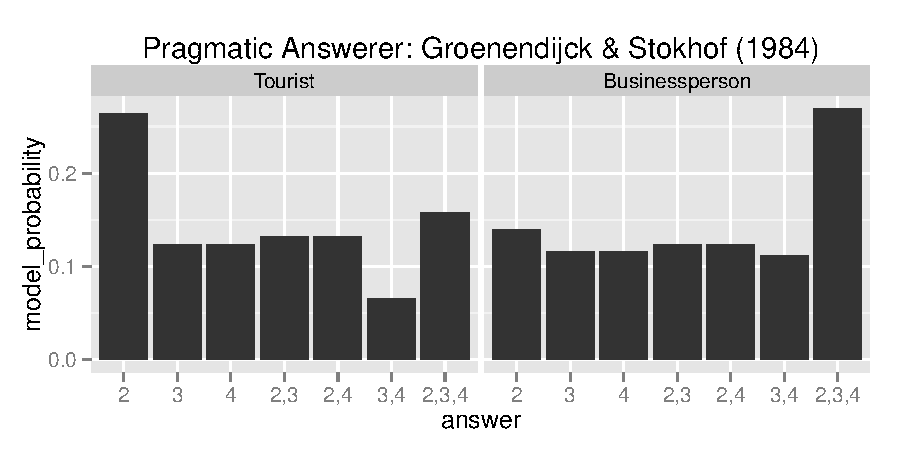
\includegraphics[scale = 1]{groenendijckPlot.pdf}
%\end{center}
%\vspace{-.25cm}
%\caption{Results for our computational experiments implementing the Groenendijck \& Stokhof (1984) \emph{mention-some} problem.}
%\label{fig:cafeExperimentResults}
%\end{figure*}

For a slightly more complex example, we consider the classic puzzle of \emph{mention-some} and \emph{mention-all} readings of wh-questions  \cite{GroenendijkStokhof84_SemanticsOfQuestions}. Some \emph{wh-}questions, like ``Who is coming to dinner tonight?'' are intended to elicit an exhaustive list of the entities that are answers. For ostensibly similar questions, like ``Where can I find a bathroom in this building?'', a mention of a single location would be sufficient. Many recent theoretical explanations in the linguistics literature appeal to questioner goals \cite<e.g.>{SchulzVanRooij06_ExhaustiveInterpretation, Ginzburg95_ResolvingQuestions}. While there are no experimental results on \emph{mention-some} and \emph{mention-all} readings with which we can compare our model's output, we include the phenomenon as a case study for its value in demonstrating how our model formalizes the standard explanation. 

We focus on a question like ``Where do they sell Italian newspapers in Amsterdam?'' that can intuitively be ambiguous between these meanings depending on who is asking: if it is a tourist, they probably just want to know the nearest place, but if it is a businessperson trying to build a newspaper distribution network, they likely want the whole list \cite<see>{GroenendijkStokhof84_SemanticsOfQuestions}. The puzzle is  one of disambiguation\footnote{Our modeling framework is compatible with another account where the `mention-some' reading is derived from the exhaustive reading via implicature \cite<e.g.>[Chapter 6]{George11_Dissertation}, but this debate lies outside the scope of this paper}: how can the same question take on different meaning in different contexts? According to our account, this happens via an inference about the questioner's underlying goal. This explanation relies on the same mechanism as the previous section, but shows how the model can operate over more complex world states and arbitrarily large spaces of possible answers.

Our world space $\mathcal{W}$ consists of all possible assignments of properties to a set of four cafes in town. Each cafe has two properties: its distance from the speaker and whether or not it sells Italian newspapers. There are two possible goals (or QUDs) $g \in \mathcal{G}$: $g_{n}$, learning the identity of the \emph{lowest-cost} cafe selling a newspaper, and $g_{a}$, learning the identity of \emph{all} cafes selling a newspaper. Both of these are represented by projections on world states, mapping a list of cafes to the single cafe selling newspapers with the lowest distance -- assuming that additional distance incurs additional cost -- or to the sublist that sell newspapers, respectively. \ndg{why talk about cost, rather than just saying closest?} The space of answers $\mathcal{A}$ is the infinite set containing all conjunctions of locations. \ndg{is that infinite? up to redundancy it's large but finite?} Again, our question space $\mathcal{Q}$ consists of a single question: ``Where can one buy an Italian newspaper?'' \ndg{what literal meaning do we assign to this question?}

For the prior $P(a)$ over answer utterances, we use a geometric distribution, which is common over spaces where probabilities should naturally scale with some count. Let $\ell(a)$ be the number of locations named in the answer (e.g. $\ell(\textrm{`none'})~=~0, \ell(\textrm{`cafe 1'})~=~1$, etc). Then the probability of an answer $a$ is given by:

$$P(a) \propto (1 - p)^{\ell(a)}p$$
In our computational experiment, we fix $p = 0.8$. 
This simple distribution has two advantageous properties: 
\begin{enumerate}[(1)]
\item the probability mass assigned to a given utterance length -- operationalized as number of conjunctions -- by the geometric distribution is spread evenly across different answers of that length.
\item we naturally assign longer answers successively lower probability, reflecting their higher cost of utterance. \end{enumerate}

\ndg{i think we can a say a lot less about this prior: just that we assume the cost of an answer is proportional to it's length, hence the prior is proportional to $\exp(length)$...}


We model the non-verbal context as affecting the questioner's goal prior $P(g)$: if they are a tourist on the street then there's a high chance that they are interested in buying a single newspaper, and hence knowing the identity of the closest shop that sells Italian newspapers ($P(g_n | c) = 0.99$); if they're a businessperson in a boardroom, then there's a high chance that they are interested in the exhaustive list of all of the Italian newspaper locations ($P(g_a | c) = 0.99$).

%\footnote{Note that this formulation of the problem differs slightly from the one given by \citeA{GroenendijkStokhof84_SemanticsOfQuestions}, although they easily map onto one another. In the original formulation, the \emph{answer} is fixed and the \emph{meaning} of the answer must be inferred to either be mention-some or mention-all. In our formulation, the meaning of each answer is unique and fixed, but the answerer must choose among a set of different possible answers. The same inferential machinery that our questioner uses to reason about which answer utterance the answerer will give could also be used to reason about which \emph{meaning} the answerer intends by their fixed utterance. The only difference is that the questioner would have uncertainty over a set of possible meanings instead of uncertainty over a set of possible answer utterances. We chose the latter because it more closely resembles the other scenarios we are modeling.}

It is unclear where these goals and goal priors may come from in real-world situations: it is likely tied to background knowledge about tourists, newspapers, and the business world, as well as past experience in social situations. While these deeper explanations lie outside the scope of our model, we still have explanatory power in showing how goals interact with other terms, and how the prior differ across scenarios. 

 \begin{figure*}[t!]
\begin{center}
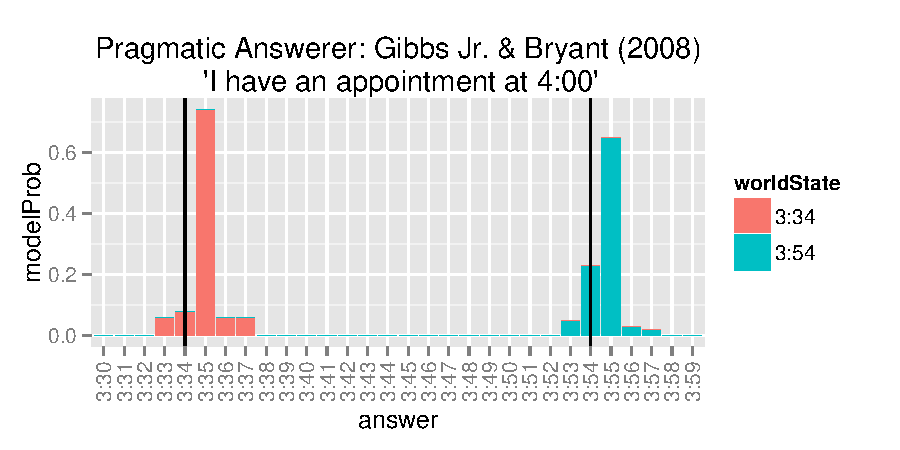
\includegraphics[scale = 1]{timeExpResults.pdf}
\end{center}
\vspace{-.25cm}
\caption{Results for our computational experiments replicating Gibbs Jr. and Bryant (2008). Vertical lines represent the true world state.}
\label{fig:timeExperimentResults}
\end{figure*}

\subsubsection{Results}

For concreteness, we set the true world to be the following :

\begin{lstlisting}
world = {`cafe1' : [3, false],
         `cafe2' : [1, true],
         `cafe3' : [3, true],
         `cafe4' : [3, true]}
\end{lstlisting}
meaning that `cafe1' is three blocks away from the speaker and does \emph{not} sell Italian newspapers, `cafe2' is one block away and \emph{does} sell Italian newspapers, and so on. We used \emph{likely-first enumeration} over the answerer model, stopping after 1000 executions of the infinite answer space (longer answers were assigned vanishingly small probability). We find that the highest probability response given the ``tourist'' context is the single location ``cafe2.'' When worlds consistent with this utterance (i.e. where cafe2 truly sells an Italian newspaper) have been projected to the closest location, the actual closest location has high probability, thus informatively fulfilling the contextually more likely goal $g_n$. Note that longer responses are unlikely for two converging reasons: they're less likely under the geometric answer prior and also may mislead the questioner into thinking another location is the closest. 

Given the ``businessperson'' context, however, the highest probability response is the conjunction ``cafe2 and cafe3 and cafe4.'' This is the exhaustive answer, informatively fulfilling the contextually more likely goal $g_a$ of knowing the location of all cafes selling Italian newspapers. Shorter answers are less likely; they are consistent with more possible worlds in the projected space, hence the projection of the true world has lower probability. 

\ndg{it occurs to me that if you ignored the question and just took the goal to be the qud you'd get the same results. maybe we'd like to have a more likely a priori goal that get's dis-preferred after hearing the question? for instance the identity goal could be a priori more likely, but then becomes less plausible after hearing the question about italian papers?}

%The literal and explicit answerers, as in the Clark scenario, do not have the means of making inferences about the questioner's underlying goals. Thus, both models incorrectly predicted that the context would not affect the preferred response. The literal answerer predicted that all combinations of cafes 2, 3, and 4 would be given in proportion to their prior likelihood (with no special preference given to the closest one). The explicit answerer predicted that the exhaustive answer would be preferred in all contexts (as this is literal semantics we encoded for the question). 
Crucially, the only difference between our model of this scenario and the Clark scenario is the richer representations of multi-dimensional world states, and the larger (unbounded) space of answers. The model itself was unchanged; we only enriched the content of its inputs. The mechanism by which goals were inferred in both cases, however, was the same: a direct function of verbal or non-verbal context. Next, we turn to a case where the world state itself provides a clue to the questioner's goal.
%%%%


\subsection{Gibbs Jr. \& Bryant (2008): Experiment 3}

It has been shown in previous work that speakers typically round their answers to the nearest 5 minute interval when asked `Do you have the time?'', even when they're wearing a digital watch \cite{DerHenstCarlesSperber02_RelevanceTellingTime}.  \citeA{GibbsBryant08_OptimalRelevance} replicated this result, and then performed a follow-up study on analog-watch wearers where they preceded their question by the context ``I have a meeting at 4:00.'' 

They found that the tendency to round times decreased as a function of the time remaining until the stated deadline: the group asked 30-16 minutes before the stated appointment rounded their responses 79\% of the time, while the group asked 14 minutes or closer to the appointment rounded significantly less (62\%). They explained this result by appealing to the questioner's goals: while an approximate time is sufficiently informative with respect to most goals, such as knowing how much time is left before heading to an appointment, a questioner who is running late may need to gauge how quickly they should move, whether they should call and warn about being late, or make other such decisions, in which case a precise time is highly relevant. 
\begin{table*}[t]
\centering
\begin{tabular}{ p{2cm} | r |||||| r }
&  \% round (Empirical) &  \% round (Model) \\
\hline
Early group &  0.79 & 0.77 \\
\hline
Late group     &0.62  & 0.60 \\
\end{tabular}
\\[1.5pt]
\caption{Comparison of our model predictions with data from Gibbs Jr. and Bryan (2008). Shows the proportion of rounding in response to ``I have an appointment at 4:00. Do you have the time?'' for two groups: an ``early group'' where the appointment was in 30-15 minutes and a ``late group'' where the appointment was in less than 15 minutes.} 
\label{table:gibbsJrExp3}
\end{table*}

To set up this scenario in our model, we take the world space to be the set of possible times, which we limit to a half hour interval (as in the experiment): $\mathcal{W}~=~\{\textrm{3:30}, \textrm{3:31}, \dots, \textrm{3:59}\}$. Unlike in the previous two case studies, where there were only two contrasting goals and two contexts that make each goal more or less likely, we now use a larger, parametrized goal space and a single context stating the time of the appointment that is held fixed across different conditions of the experiment. 

This goal space $\mathcal{G}$ includes the trivial projection $g_0(w) = w$, corresponding to the context-independent goal of learning the true time, in addition to a set of goals parameterized by a threshold time $\tau$, representing the point at which the agent believes they are running late to their appointment (likely based on expectations about travel time, social norms concerning lateness, and other exogenous factors). If the agent has goal $g_\tau$ for a given $\tau$, then for times $t < \tau,$ the agent only cares about the approximate time, rounded to the nearest 5 minute increment, in order to know roughly how much time they have before leaving. For times $t > \tau$, the agent cares about the exact time in order to make the kind of decisions described above. Formally,

\DeclarePairedDelimiter{\floor}{\lfloor}{\rfloor}

$$g_\tau(w) = \left\{
\begin{array}{rcl}
w & & w \ge \tau\\
5\floor{\frac{w}{5} + \frac{1}{2}} & & w < \tau;  \\
\end{array}
\right.
$$
where $\floor{w}$ returns the \emph{floor} of an integer and all operations are assumed to act on the minutes component of a time $w$. For example, the goal $g_{3:50}$ with the threshold set at $\tau = $3:50 corresponds to a projection function that rounds input worlds earlier than 3:50 and does not round worlds later than 3:50. This would be the case if the agent knew they would need to leave around 3:50 in order to make it to an appointment on time. 

The goal prior $P(g_\tau)$ assigns probability $p=0.25$ to the context-independent goal $g_0$ of wanting to know the exact time. The remaining probability mass is divided across different threshold goals ($\tau \in \{$ 3:31, 3:32, \dots, 3:59 $\}$) according to the following rule: the likelihood of each goal $g_\tau$ is inversely proportional to the distance (in minutes) between the threshold $\tau$ and the given appointment time $c$, reflecting the intuition that the questioner will be more likely to be running late, and therefore in need of the exact time, as it approaches the appointment time:

$$P(g_0) = 0.25$$
$$P(g_\tau; c) = \frac{0.75}{\sum_{i=1}^{29}i}(30 - |\tau - c|)$$

The set of answers is the set of times that could be given (e.g. 3:30, 3:31, \dots, 4:00), with multiples of 5 preferred:
$$P(t) = \left\{
\begin{array}{lcl}
0.125 & & t \equiv 0 \mod 5 \\
0.01 & & \textrm{otherwise} \\
\end{array}
\right.
$$ As \citeA{GibbsBryant08_OptimalRelevance} point out, their participants all wore analog watches, hence precise answers have higher cost. In fact, an earlier study in the same paper showed that in the absence of any context, participants wearing analog watches responded with rounded answers 90\% of the time, so this prior is realistic. 

For our answers, we use exact number semantics: the response ``3:35'' evaluates to true in worlds where the time is in fact 3:35, and false otherwise. While we suppressed \emph{a priori} false answers for convenience in other case studies (they would be naturally be assigned vanishingly small probability anyway), note that we cannot do so here: answerers must be allowed to make \emph{a priori} false utterances that get reinterpreted by the listener to be true under the QUD \cite<see>{KaoWuBergenGoodman14_NonliteralNumberWords}. 

%\todo[inline]{return to this in the discussion}

 \subsubsection{Results}
 
To compare our model's performance against the `early group' and `late group' conditions in \citeA{GibbsBryant08_OptimalRelevance}, we ran two simulations. In both, the context is ``I have an appointment at 4:00.'' In the first, the true world state is between 3:30 and 3:45 (the `early' condition); in the second, the true world state is between 3:45 and 3:59 (the `late' condition). In each condition, we ran our pragmatic answerer model for all true worlds in the appropriate range of times, and report the average probability of responding with a rounded answer. Our results are compared against empirical data from Gibbs Jr. and Bryant \citeyear{GibbsBryant08_OptimalRelevance} in Table \ref{table:gibbsJrExp3}. 

To more closely analyze what is driving our model's performance in these two conditions, we examine the answer behavior for two specific world states: one from the `early group' (3:34) and one from the `late group' (3:54). Answer probabilities for these two conditions are shown in Figure \ref{fig:timeExperimentResults}. We found that our pragmatic answerer model rounds the 3:34 to 3:35 in the `early' condition with probability $p = 0.74$, but rounds 3:54 to 3:55 with lower probability $p = 0.65$ in the `late' condition. 

The goal prior is the key component of the model governing this difference. Note that that (1) \emph{all} states in the pre-image of the rounding projection from the true time $t_0$ are assigned lower probability than the rounded time $g_\tau(t_0)$, due to the influence of goals $g_\tau$ with thresholds $\tau > t_0$ and (2) the true time $t_0$ is assigned relatively higher probability than the other non-rounded times, due to the influence of the pure goal $g_0$ and goals $g_\tau$ with thresholds $\tau < t_0$. This dynamic, paired with the upward-skewed prior on goal priors discussed above, causes the `late' condition to assign a much higher relative probability to the true time, than the `early' condition. The pragmatic answerer thus accurately captures the empirical results both qualitatively and quantitatively. 

%Our literal and explicit answerer models fail to capture these contextual differences, as they do not reason about the space of underlying goals (which justify rounding) and always give the exact time. The literal answerer always gives the exact time because it is the only property of the world, which they are attempting to be informative about without regard to the question. The explicit answerer always gives the exact time because it uses the explicit question meaning, which simply asks for the time.

%\todo[inline]{rdh: Actually, in the experiment the question was ``Do you have the time?'' to which the literal and explicit answers would be ``yes'' or ``no'', right? We don't allow these responses in our model because they're not what we're interested in (i.e. \emph{no one} responded this way), but they are the kinds of answers our literal and explicit answerers would give}

\end{document}  
